\documentclass[preprint,12pt,authoryear]{elsarticle}
% ---------------------------------------------------------------------------
% International Journal of Information Management -- research article
% Set \anontrue to produce the anonymised manuscript for double-blind review.
% ---------------------------------------------------------------------------
\newif\ifanon
\anontrue
\usepackage[utf8]{inputenc}
\usepackage[T1]{fontenc}
\usepackage{lmodern}
\usepackage{amsmath,amssymb,amsthm,mathtools}
\usepackage{graphicx}
\usepackage{booktabs}
\usepackage{tabularx}
\usepackage{multirow}
\usepackage{array}
\usepackage{enumitem}
\usepackage{lineno}
\usepackage{xcolor}
\usepackage{placeins}
\usepackage[labelfont=bf]{caption}
\usepackage[a4paper,margin=2.5cm]{geometry}
\usepackage[colorlinks=true,linkcolor={blue!55!black},citecolor={green!40!black},urlcolor={blue!60!black}]{hyperref}
\bibpunct{(}{)}{;}{a}{,}{,}
\providecommand{\doi}[1]{\url{https://doi.org/#1}}
\newcolumntype{L}{>{\raggedright\arraybackslash}X}
\newcolumntype{C}{>{\centering\arraybackslash}X}
\newcolumntype{P}[1]{>{\raggedright\arraybackslash}p{#1}}
\newcommand{\E}{\mathbb{E}}
\newcommand{\pt}{\,pt}
\newtheorem{proposition}{Proposition}
\theoremstyle{definition}
\newtheorem{assumption}{Assumption}
\renewcommand{\arraystretch}{1.12}
\renewcommand{\topfraction}{0.95}
\renewcommand{\bottomfraction}{0.9}
\renewcommand{\textfraction}{0.05}
\renewcommand{\floatpagefraction}{0.7}
\setcounter{topnumber}{3}
\setcounter{totalnumber}{5}
\setlength{\tabcolsep}{4pt}
\journal{International Journal of Information Management}

\begin{document}
\begin{frontmatter}

\title{Managing evidence, not ideas: A convergence-based design of experimentation information systems for digital services in the age of generative AI}

\ifanon\else
\author[kozminski]{Pawe{\l} Kura{\'s}\corref{cor1}}
\ead{pkuras@kozminski.edu.pl}
\author[prz]{Ewelina Nycz}
\ead{e.nycz@prz.edu.pl}
\author[prz]{Patryk Organi{\'s}ciak}
\ead{org@prz.edu.pl}
\cortext[cor1]{Corresponding author.}
\affiliation[kozminski]{organization={Kozminski University},
  addressline={ul. Jagiello\'nska 57/59}, postcode={03-301}, city={Warsaw}, country={Poland}}
\affiliation[prz]{organization={Rzesz\'ow University of Technology},
  addressline={al. Powsta\'nc\'ow Warszawy 12}, postcode={35-959}, city={Rzesz\'ow}, country={Poland}}
\fi

\begin{abstract}
Digital services are improved through loops of ideation, deployment and online testing, and generative AI is making ideation almost free. Whether such loops improve what organisations ship depends on how they manage the evidence that tests produce. Building on a convergence theorem for the iterate--test loop of design thinking, we derive eight design principles for experimentation information systems and instantiate them in an evidence ledger, which retains every tested variant with its evidence, re-tests the leading variants and ships on a lower confidence bound. We evaluate the artefact in a programmable testbed: a queueing model of a twelve-feature digital service, validated against a discrete-event emulation of its network topology, with 51 service instances and more than fifty thousand simulated improvement projects. Under equal traffic the ledger ships configurations worth 94.7--95.1\% of the attainable optimum, 7.9 to 16.7 percentage points more than a sequence of champion--challenger A/B tests ($p<0.001$ on every landscape class), and it reduces the loss from choosing among tested variants, and the overestimation of the chosen one, by a quarter to a third. The validity of screening ideas, not their number, governs what generative ideation adds. Biases favouring the incumbent or new variants are harmless below the noise of a test, whereas persistent instrumentation bias survives re-testing and requires an audit. Forgetting pays only after abrupt shifts, and a Pareto archive represents disagreeing stakeholders better than fixed weights. Evaluation, not generation, is the scarce resource that experimentation information systems must manage.
\end{abstract}

\begin{keyword}
online experimentation \sep A/B testing \sep design science \sep generative AI \sep decision making \sep design thinking
\end{keyword}
\end{frontmatter}

\linenumbers

% ===========================================================================
\section{Introduction}
\label{sec:intro}

Organisations that run digital services have turned product development into a stream of experiments. A change to a web shop, a public e-service or a mobile app is deployed behind a feature flag, exposed to a slice of traffic, measured, and kept or rolled back \citep{kohavi2009, kohavi2020, fabijan2017}. The practice has a managerial philosophy behind it, variously called design thinking, lean experimentation or the scientific approach to decisions \citep{brown2008, ries2011, camuffo2020, thomke2020}, and a growing body of evidence that firms which experiment more perform better \citep{brynjolfsson2016, koning2022}. Generative artificial intelligence now promises to remove the last bottleneck of the stream by producing ideas, copy and even working variants at negligible cost \citep{dwivedi2023, girotra2023, noy2023}.

Whether the stream actually improves what organisations ship is an information management question. Each experiment produces evidence of limited precision, and the organisation has to decide where to spend its limited traffic, which variants to keep, how to combine the results of tests run at different times and how far to trust the apparent winner. Practice offers rules of thumb for single experiments, such as significance thresholds, minimum sample sizes and guards against peeking \citep{kohavi2020, johari2022}, but little guidance on managing the evidence of a whole sequence of experiments, and the sequence is where most value is created or lost. The apparent winner of many noisy comparisons is overrated \citep{smithwinkler2006, lee2018}, a single significant test is a weak basis for a launch \citep{gelman2014, azevedo2020}, and a stream of ideas from a language model multiplies the number of comparisons without making any of them more precise.

A recent preprint \citep{kuras2026} gives this question a theoretical anchor. It models the iterate--test core of design thinking as search over a finite space of prototypes whose utility is learned from noisy tests, and proves that the prototype a team believes to be best is eventually a local optimum when five conditions hold: the frame is finite, ideation is local, improving ideas keep coming, tests are unbiased and repeated, and nothing tested is discarded. The theorem is stated for design teams and evaluated on abstract landscapes. It does not say how an organisation should build the information system that runs the loop, nor how much the conditions matter in a realistic digital service, where tests are online experiments on live traffic, test noise depends on sample size, and generative AI changes the supply of ideas.

We address that gap with a design science study \citep{hevner2004, gregor2013, peffers2007}. Our research question is: \emph{How should an experimentation information system manage the evidence produced by iterative online testing so that a digital service reliably improves, and how does generative ideation change the answer?} We make four contributions.

\begin{enumerate}[leftmargin=*,itemsep=2pt]
\item We translate the convergence theorem and its corollaries into eight design principles for experimentation information systems (XIS), each tied to the condition of the theorem it secures, and instantiate them in an \emph{evidence ledger}: a component that keeps every tested variant with a calibrated belief and an evidence count, plans re-tests of the leaders, and ships on a lower confidence bound (Section~\ref{sec:design}).
\item We build a programmable testbed for evaluating such systems. It represents a digital service with twelve deployable capabilities, a network topology of edge, firewall, load balancer, application pool, cache, database, ML inference and an external language-model API, two user segments, and an experimentation plane of feature flags, telemetry and a data store. A queueing model gives the exact utility of all $2^{12}$ configurations; a discrete-event emulation of the topology validates the model and the statistical test sampler (Section~\ref{sec:method}).
\item We report nine experiments with more than fifty thousand simulated improvement projects on 51 service instances. They quantify the cost of choosing among tested variants and the optimiser's curse, compare the ledger with experimentation-governance practices under one traffic budget, locate the best split of traffic between new variants and re-tests, separate the volume of generative ideation from the validity of its screening, map which measurement biases matter, and examine drifting criteria, abrupt shifts and disagreeing stakeholders (Section~\ref{sec:results}).
\item We draw implications for information management research and practice. The central one is that evaluation, not generation, is the scarce resource: as generative AI makes ideas cheap, the value of an experimentation programme is set by how it manages evidence (Section~\ref{sec:discussion}).
\end{enumerate}

% ===========================================================================
\section{Theoretical background}
\label{sec:background}

\subsection{Online experimentation as an information management problem}

Controlled online experiments, or A/B tests, are the standard method by which digital firms evaluate changes \citep{kohavi2009, kohavi2020}. Continuous experimentation embeds them in the delivery pipeline, so that features are deployed behind flags and evaluated on live traffic \citep{bosch2012, fitzgerald2017, fabijan2017}; a recent review of 128 studies catalogues its processes, infrastructure and cultural, statistical and ethical challenges \citep{auer2021}. A mature experimentation platform is an information system in its own right: it assigns users to variants, collects telemetry, computes metrics, stores results and supports decisions. The information systems literature has studied the value of data-driven decision making and of analytics capabilities in general \citep{brynjolfsson2016, provost2013, gupta2016, duan2019, mikalef2021}, but the experimentation platform has mostly been treated as plumbing, and the decision logic that sits on top of it, that is, which variants to test, how often and how to choose among them, has been left to rules of thumb.

Those rules address one experiment at a time. Practitioners are warned against peeking at interim results \citep{johari2022}, against sample-ratio mismatch and other data-quality problems \citep{fabijan2019}, against misreading metrics \citep{dmitriev2017}, against the highest paid person's opinion (HiPPO) overriding data \citep{kohavi2009}, and against novelty effects that inflate the early results of a new variant \citep{kohavi2020}. A programme of experiments raises problems that no single experiment shows. When many variants are compared, the winner's estimated effect is biased upwards \citep{lee2018}, the more so the noisier the tests; with heavy-tailed effects most tests find nothing and a few find much \citep{azevedo2020}; and a significance threshold controls false positives per test, not the quality of the configuration that a sequence of tests eventually ships. Variance-reduction techniques make each test more precise \citep{deng2013}. Bandit algorithms allocate traffic adaptively among a fixed set of arms \citep{scott2015, russo2018}, also in marketing practice \citep{schwartz2017}, and best-arm identification asks how to find the best of them with few samples \citep{russo2020}, but neither addresses a set of arms that grows as new ideas arrive and are built.

\subsection{Search, evaluation and the iterate--test loop}

Simon described design as search for a satisfactory alternative under bounded rationality \citep{simon1996}. Organisation theory has modelled search on rugged landscapes, where local adaptation finds a nearby peak and misses distant ones \citep{levinthal1997, march1991, kauffman1993}, and has shown that imperfect evaluation of alternatives shapes the outcome as much as their generation \citep{knudsen2007}, sometimes beneficially, since a noisy evaluator can leave a local peak that an accurate one would not. Experiments on idea generation point the same way: groups that produce more ideas do not select better ones, and the quality of the best idea depends on the ability to recognise it \citep{girotra2010}. Building several prototypes in parallel before feedback improves design outcomes \citep{dow2010}, and design thinking is argued to work by disciplining judgement \citep{liedtka2015, micheli2019}.

\citet{kuras2026} formalise the iterate--test core of design thinking. Within a fixed frame, a prototype is a subset $p$ of a finite set of features $F$ with an unknown utility $U(p)\in[0,1]$. In each round a team proposes variants of what it has built, builds one, tests it and some older prototypes, and updates its beliefs $M^p_k$; the favourite is the prototype with the highest belief. A test returns $y=U(p)+b_k+\varepsilon_k$ with noise of variance at most $\sigma^2$ and a bias $|b_k|\le B$. Their main results, restated in the vocabulary of this paper, are the following.

\begin{enumerate}[leftmargin=*,label=(T\arabic*),itemsep=2pt]
\item \emph{Convergence.} If the frame is finite (A1), ideas are variants of what has been built (A2), the chance of building an improving variant is not summable (A3), tests are unbiased and every retained prototype is re-tested infinitely often (A4), and no tested prototype is discarded (A5), then almost surely the favourite is eventually a single locally optimal prototype and the belief about it converges to its utility.
\item \emph{Bias.} With bias bounded by $B$, the eventual favourites are $2B$-locally optimal: no variant beats them by more than $2B$.
\item \emph{Drift.} If the criteria drift within a band of half-width $D$, the eventual favourites are $2D$-locally optimal for the reference criteria and $4D$-locally optimal for the current ones.
\item \emph{Stakeholders.} With several stakeholders and an archive of non-dominated prototypes, the archive converges to a locally Pareto-optimal set.
\end{enumerate}

\noindent Their simulations add that the limit is remote at realistic horizons, that teams overrate the prototype they choose (the optimiser's curse; \citealp{smithwinkler2006}), that a budget spent entirely on new prototypes is wasteful, that a bias towards the favourite is harmless until it is as large as the noise of a test, and that rough pre-screening of ideas is worth more than the choice of testing policy.

The theorem is a kernel theory in the sense of design science \citep{gregor2007, gregor2020}: it states conditions under which a class of processes achieves a goal, and each condition can be secured or violated by the information system that runs the process. Three features of real digital services, however, are absent from the abstract model. Test noise is not a constant but a consequence of how much traffic a test receives, and traffic is the budget. Utility is not an arbitrary landscape but emerges from the interaction of features with a service topology under load, so that a feature's value depends on capacity. And the supply of ideas is changing: language models produce many ideas quickly \citep{girotra2023, boussioux2024}, raise the quality of individual output \citep{noy2023, dellacqua2023} and can act as judges of quality \citep{zheng2023}, but also make output more alike \citep{doshi2024}. Whether the theory's guidance survives these features, and how large the stakes are, is an empirical question about the artefact, which we answer in a testbed.

% ===========================================================================
\section{Design of the evidence-ledger experimentation information system}
\label{sec:design}

\subsection{From conditions to design principles}

Following \citet{gregor2020}, a design principle states what a system should enable, for whom and why. We derive eight principles (Table~\ref{tab:dp}, Figure~\ref{fig:framework}). Five secure the conditions of the convergence result, and three follow from its corollaries and from the finite-horizon findings of \citet{kuras2026}.

\begin{figure}[!tbp]
\centering
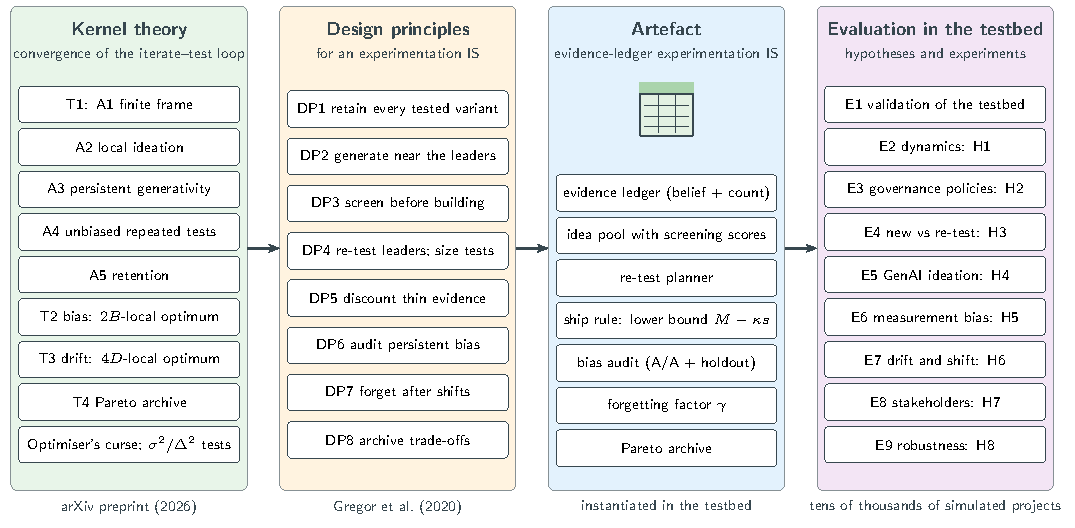
\includegraphics[width=\textwidth]{figures/fig_framework.pdf}
\caption{Research framework. Conditions and results of the convergence theorem (kernel theory) are translated into design principles, the principles are instantiated in the evidence-ledger artefact, and the artefact is evaluated in nine experiments that test hypotheses H1--H8. Schematic drawn in TikZ with code written with the assistance of Claude (Anthropic).}
\label{fig:framework}
\end{figure}

\begin{table}[!tbp]
\caption{Design principles for an experimentation information system, the theoretical condition each secures, its instantiation in the evidence ledger, and where it is evaluated.}
\label{tab:dp}
\centering\footnotesize
\begin{tabularx}{\textwidth}{@{}P{0.75cm}LP{2.0cm}LP{0.95cm}@{}}
\toprule
DP & Principle (the XIS should \ldots) & Kernel theory & Instantiation in the ledger & Exp.\\
\midrule
DP1 & retain every tested variant with its full evidence record & A5 retention & ledger of beliefs and evidence counts & E2, E3\\
DP2 & generate new variants near the current leaders, every round & A2, A3 & idea pool fed by variants of leaders & E3, E5\\
DP3 & screen ideas before spending traffic on them & speed of discovery & screening score per idea; build the best-screened & E5\\
DP4 & keep building, re-test the leaders and size tests to the signal & A4; $\sigma^2/\Delta^2$ & build rate; re-test planner; test-size choice & E3, E4, E11\\
DP5 & discount thin evidence when choosing what to ship & optimiser's curse & ship on $M-\kappa s$ & E2, E3\\
DP6 & audit measurement for persistent bias & T2 ($2B$) & A/A-style bias audit & E6\\
DP7 & bound drift, and forget old evidence after shifts & T3 ($4D$) & forgetting factor $\gamma$ & E7\\
DP8 & keep trade-offs open when stakeholders disagree & T4 & archive of non-dominated variants & E8\\
\bottomrule
\end{tabularx}
\end{table}

\emph{DP1 Retention.} Experimentation platforms typically archive results per experiment, and a sequence of champion--challenger tests keeps only the current champion and its latest result. The theorem needs the opposite: every tested variant stays available as a rival, with all its evidence pooled. \emph{DP2 Local and persistent generation.} New variants should be proposed near the leaders in every round; in our artefact the product team, possibly assisted by a language model, proposes $V$ variants of a randomly chosen leader. \emph{DP3 Screening.} Building and testing a variant costs traffic, whereas a rough judgement of its promise costs little; the ledger records a screening score for every idea and builds the idea with the best score among all those not yet built. \emph{DP4 Repeated testing.} Beliefs become correct only if leaders are tested again; the planner re-tests the three leading variants and one variant in rotation in every round, and the size of a test, which sets its noise, is a design choice. \emph{DP5 Discounting thin evidence.} Because the favourite is selected for its high estimate, its estimate is biased upwards; the ledger ships the variant with the highest lower bound $M^p_k-\kappa s^p_k$, where $s^p_k$ is the posterior standard deviation, with $\kappa=1$. \emph{DP6 Bias audit.} Re-testing removes noise, not bias, so persistent measurement bias must be estimated separately, for example by A/A-style comparisons of instrumented and server-side measurements. \emph{DP7 Drift.} Bounded drift of criteria costs a bounded amount, while an abrupt change of the environment makes old evidence misleading; a forgetting factor $\gamma\le1$ discounts old evidence. \emph{DP8 Stakeholders.} When users, operations and finance weigh criteria differently, the ledger can keep an archive of non-dominated variants instead of a single favourite.

\subsection{The artefact}

The evidence ledger sits in the experimentation plane of a digital service (Figure~\ref{fig:topology}) and runs the cycle of Figure~\ref{fig:cycle}. In round $k$ it (1) collects $V$ ideas for variants of a leader, (2) scores them, (3) deploys the best-screened unbuilt idea behind a feature flag, (4) runs one test of $n$ sessions on the new variant and re-tests three leaders and one rotating variant, (5) receives the measured criteria from telemetry, (6) updates conjugate normal beliefs with prior mean $0.5$ and variance $0.08$ and known test variance $\sigma^2(n)$, (7) plans the next re-tests and (8) decides whether to continue or ship. A round thus consumes five tests. Apart from the ship rule, the procedure is the design-thinking loop of \citet{kuras2026}, which lets us attribute differences between the two to DP5.

\begin{figure}[!tbp]
\centering
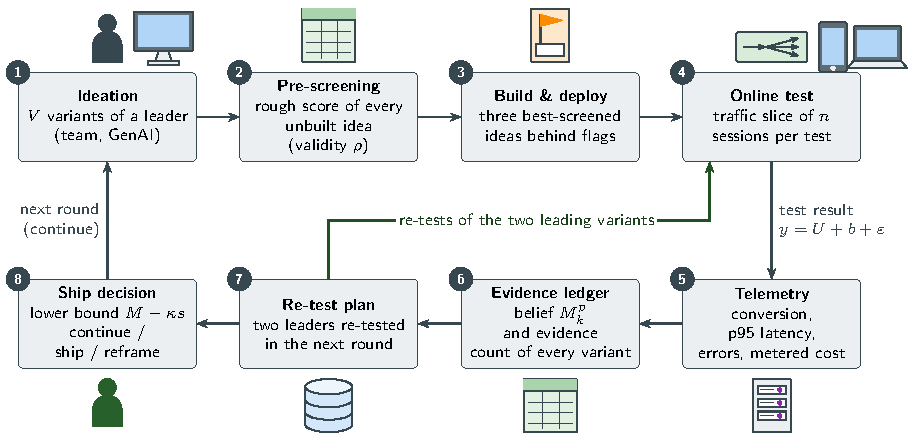
\includegraphics[width=0.92\textwidth]{figures/fig_cycle.pdf}
\caption{One round of the evidence-ledger loop. Steps 1--3 generate, screen and deploy a variant; steps 4--6 test it and update the evidence; steps 7--8 plan re-tests and decide. The green path returns the leaders to the next round's tests. Schematic drawn in TikZ with code written with the assistance of Claude (Anthropic).}
\label{fig:cycle}
\end{figure}

\subsection{The ledger as an information system}
\label{sec:ledgeris}

The ledger is an information system, not only a decision rule. It stores, for every variant ever deployed, its configuration, its screening score, every test result with its time and sample size, the current belief and its uncertainty, and the evidence count; it presents this record to the product team as a ranked list in which each belief is shown with its uncertainty; and it turns the record into three kinds of proposal, namely which idea to build, which variants to re-test and which variant could be shipped. The decisions themselves remain with people: the team decides what counts as a variant, whether to accept a proposal to ship, when to reframe and how to weigh the criteria, and it supplies the screening judgement. Table~\ref{tab:anatomy} sets out the resulting design theory in the eight components of \citet{gregor2007}.

\begin{table}[!tbp]
\caption{The evidence ledger as a design theory, following the components of \citet{gregor2007}.}
\label{tab:anatomy}
\centering\footnotesize
\begin{tabularx}{\textwidth}{@{}P{3.4cm}L@{}}
\toprule
Component & Content in this study\\
\midrule
Purpose and scope & Improve what a digital service ships from a programme of online experiments, within one framing of the problem\\
Constructs & variant, test, belief, evidence count, screening score and validity, leader, favourite, ship bound, bias, drift, archive\\
Principles of form and function & DP1--DP8 (Table~\ref{tab:dp})\\
Artefact mutability & number of leaders, rotation, $\kappa$, forgetting factor, archive versus single favourite, audit size are configurable\\
Testable propositions & H1--H8 (Section~\ref{sec:hyp})\\
Justificatory knowledge & convergence theorem and corollaries \citep{kuras2026}; optimiser's curse \citep{smithwinkler2006}; best-arm identification \citep{russo2020}\\
Principles of implementation & pool evidence across experiments; display beliefs with uncertainty; keep humans responsible for framing, screening and the decision to ship; audit instrumentation\\
Expository instantiation & Python implementation in the testbed (Section~\ref{sec:method}); ledger excerpt in Table~\ref{tab:vignette}\\
\bottomrule
\end{tabularx}
\end{table}

Table~\ref{tab:vignette} shows what the ledger displays after 100 tests in one run on the reference service. The current favourite has the highest belief (0.94), but it rests on three tests and its true utility is 0.78, a typical case of the optimiser's curse. The second variant has a lower belief (0.77) resting on sixteen tests and is worth 0.73. Shown with their uncertainty and evidence counts, the two are no longer simply first and second: the favourite is a promising but unconfirmed variant, and the ledger's next round re-tests it. In this snapshot the lower bound still favours it (0.87 against 0.74); after further re-tests its belief falls towards its true value. The idea the screen ranks third is in fact the best of the three, which illustrates why screening validity matters.

\begin{table}[!tbp]
\caption{Excerpt of the ledger after 100 tests in one run on the reference service (tests of 2,000 sessions, $\sigma=0.12$). The true utilities, unknown to the team, are shown for illustration; $U^*=0.881$.}
\label{tab:vignette}
\centering\footnotesize
\setlength{\tabcolsep}{3pt}
\begin{tabularx}{\textwidth}{@{}LP{1.0cm}P{0.8cm}P{0.85cm}P{1.25cm}P{1.0cm}@{}}
\toprule
Variant (enabled capabilities) & Belief & s.d. & Tests & Bound $M-s$ & True $U$\\
\midrule
COMP, CACHE, REPL, RECO, ONECLICK, AUTOC, TELEM & 0.940 & 0.067 & 3 & 0.873 & 0.782\\
COMP, CACHE, REPL, RECO, CHAT, ONECLICK, AUTOC, PRIV & 0.773 & 0.030 & 16 & 0.743 & 0.725\\
COMP, CACHE, REPL, ONECLICK, TELEM & 0.735 & 0.042 & 8 & 0.693 & 0.610\\
COMP, CACHE, REPL, RECO, CHAT, ONECLICK, PRIV & 0.724 & 0.081 & 2 & 0.643 & 0.682\\
\midrule
\multicolumn{6}{@{}p{\linewidth}@{}}{\raggedright\textit{Best-screened unbuilt ideas} (screening score; true $U$): COMP, CACHE, REPL, ONECLICK, AUTOC, TELEM (1.13; 0.646); COMP, CACHE, CHAT, ONECLICK (1.11; 0.643); COMP, CACHE, REPL, RECO, CHAT, ONECLICK, AUTOC, TELEM (1.02; 0.802).}\\
\bottomrule
\end{tabularx}
\end{table}

Because the ledger records each built idea's screening score next to its first test result, it can also estimate the validity of its own screening: the correlation between the two, divided by the square root of the reliability of a single test, estimates $\rho$ among the ideas the team actually builds (Section~\ref{sec:discussion}).

\subsection{Hypotheses}
\label{sec:hyp}

The theory and the preprint's simulations lead to eight hypotheses about the artefact in a digital service.

\begin{description}[leftmargin=*,itemsep=2pt,font=\normalfont\itshape]
\item[H1 (cost of choosing).] At realistic budgets the shipped configuration falls short of the best configuration already tested, and its believed utility exceeds its true utility; discounting thin evidence (DP5) reduces both.
\item[H2 (governance).] Under the same traffic, policies that retain and re-test (DP1, DP4) ship better configurations than champion--challenger A/B testing.
\item[H3 (allocation).] Shipped utility has an interior optimum in the share of tests spent on new variants, and the optimum moves towards re-testing as tests become noisier.
\item[H4 (generative ideation).] The validity of screening contributes more to shipped utility than the number of ideas generated, and homogenised ideas reduce shipped utility.
\item[H5 (bias).] Biases that favour the incumbent or new variants are harmless while smaller than the noise of a test; persistent instrumentation bias degrades outcomes and is not removed by re-testing.
\item[H6 (drift).] Under bounded drift the loop keeps tracking the moving optimum; forgetting improves recovery after an abrupt shift but costs under stationarity.
\item[H7 (stakeholders).] At equal budget an archive of non-dominated variants covers the stakeholders' Pareto front better than loops with fixed weights.
\item[H8 (robustness).] The ledger's advantage over champion--challenger testing holds across services, budgets, test sizes and ideation settings, and grows with test noise.
\end{description}

% ===========================================================================
\section{Method: a programmable testbed}
\label{sec:method}

Evaluating an experimentation system on a live service would require the same service to be improved many times under different policies, which is impossible, and would not reveal the true utility of what is shipped. We therefore evaluate the artefact in an artificial but validated setting, a choice that design science recognises for early, technically oriented evaluation \citep{venable2016} and whose simulation-based benchmarking against competing artefacts is an established evaluation pattern in IS design research \citep{prat2015} and that management research uses to develop theory where processes are path dependent \citep{davis2007, harrison2007}. In the terms of FEDS, this is a summative evaluation in an artificial setting whose purpose is to establish the efficacy of the design principles and their robustness to the conditions a real service would impose, before a naturalistic evaluation with practitioners; the risk it addresses first is technical (whether the principles improve outcomes at all), and the main remaining risk, that teams do not use the ledger as intended, is left to that later evaluation (Section~\ref{sec:discussion}). The testbed is written in Python, uses fixed random seeds, and is released with all scripts and raw outputs \citep{dataset2026}.

\subsection{The digital service and its topology}
\label{sec:service}

The testbed represents an online retail service (Figure~\ref{fig:topology}). Users arrive as a Poisson stream of $\lambda=30$ sessions per second, 62\% on mobile devices with a round-trip time of 65\,ms and 12\,Mbit/s, the rest on desktop with 28\,ms and 60\,Mbit/s. A request passes the Internet, an edge router (or a content delivery network, CDN, when enabled), a web-application firewall, a core switch and a load balancer, and is served by a pool of $c=9$ application workers. A worker is held for the whole synchronous request, including database calls (an M/M/3 server of 4\,ms), calls to an ML inference pool of six workers and, if enabled, an external language-model API. Telemetry flows to a collector and an experiment data store; feature flags are set by the experiment server.

\begin{figure}[!tbp]
\centering
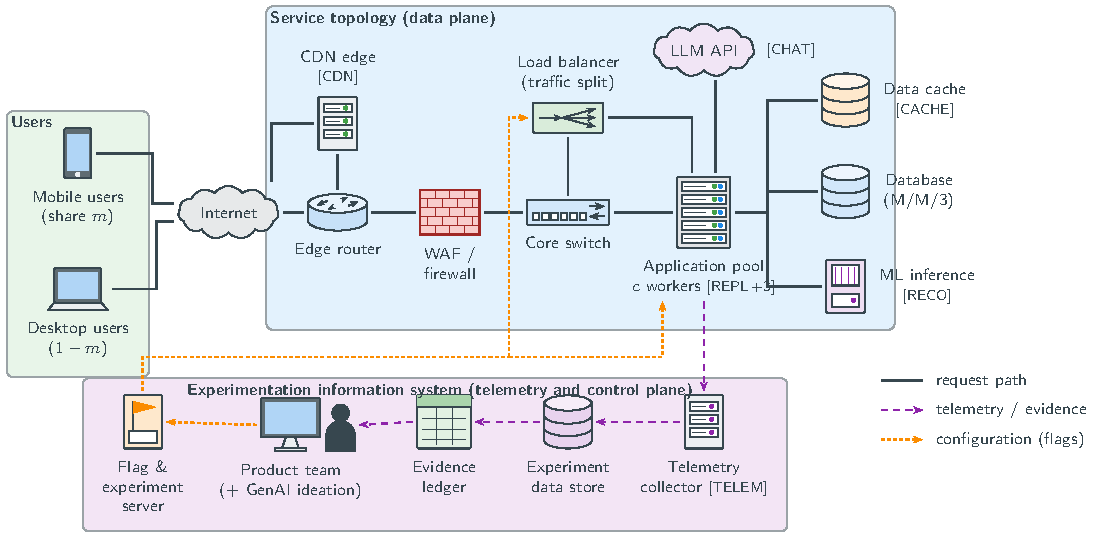
\includegraphics[width=\textwidth]{figures/fig_topology.pdf}
\caption{Topology of the testbed. The data plane serves user requests; deployable capabilities are shown in brackets at the components they change. The experimentation information system (bottom) receives telemetry, keeps the evidence ledger and sets feature flags that route a slice of traffic to the variant under test. Schematic drawn in TikZ with code written with the assistance of Claude (Anthropic).}
\label{fig:topology}
\end{figure}

A configuration of the service is a subset of twelve deployable capabilities (Table~\ref{tab:features}), giving $2^{12}=4{,}096$ configurations. Each capability changes some of the following: the CPU time of a request, the number of database calls, ML inference time, page weight, pages per session, the number of workers, conversion in each user segment, fixed and per-session cost, operational complexity and the rate of fraud losses. Six pairwise interactions encode dependencies that practitioners will recognise: recommendations need behavioural telemetry, step-up authentication defeats one-click checkout, and a privacy dashboard offsets the friction of authentication and telemetry. Capacity creates further interactions, since capabilities that add work per request push the application pool towards saturation unless caching or replicas relieve it.

\begin{table}[!tbp]
\caption{Deployable capabilities of the reference service and their main mechanisms. Lifts are changes of log-conversion for mobile/desktop users; costs are per hour unless stated.}
\label{tab:features}
\centering\footnotesize
\begin{tabularx}{\textwidth}{@{}P{1.95cm}P{3.3cm}LL@{}}
\toprule
Flag & Capability & Load and latency & Experience, cost and risk\\
\midrule
CDN & edge content delivery & shorter round trips; offloads static requests & cost 420\\
COMP & response compression & page weight $\times0.72$; +3\,ms CPU & complexity 0.3\\
CACHE & application data cache & database calls $\times0.35$ & cost 180\\
REPL & three extra replicas & $c\to c+3$ workers & cost 900\\
RECO & ML recommendations & +25\,ms ML inference per page & lift $+0.03/{+0.04}$; +0.095 with TELEM; cost 1{,}500\\
CHAT & GenAI shopping assistant & external API delay & lift $+0.02/{+0.06}$; 0.045 per session\\
ONECLICK & one-click checkout & one page fewer per session & lift $+0.15/{+0.12}$; fraud $\times1.25$\\
MFA & step-up authentication & +2\,ms CPU & lift $-0.08/{-0.06}$; fraud $\times0.25$; $-0.11$ with ONECLICK\\
MEDIA & rich product media & page weight $\times2$ & lift $+0.03/{+0.085}$; cost 250\\
AUTOC & search autocomplete & +3.5\,ms CPU; 0.3 pages fewer & lift $+0.02/{+0.05}$\\
PRIV & privacy dashboard & --- & lift $+0.02$; offsets MFA and TELEM friction\\
TELEM & behavioural telemetry & +4\,ms CPU & lift $-0.015$; cost 600; enables RECO\\
\bottomrule
\end{tabularx}
\end{table}

\subsection{Criteria and utility}

Each configuration is judged by the three criteria of design thinking \citep{brown2008}. \emph{Desirability} $U_{\mathrm d}$ is the expected conversion rate, which falls exponentially once the mean page time of a session exceeds one second and with the error rate. \emph{Feasibility} $U_{\mathrm f}$ combines a service-level objective on the 95th percentile of page-load time (2.6\,s) with operational complexity. \emph{Viability} $U_{\mathrm v}$ is the hourly profit after fraud losses and infrastructure, bandwidth and per-session costs. Desirability and viability are scaled to $[0,1]$ over the configurations that do not saturate any tier, and the utility is $U=0.45U_{\mathrm d}+0.25U_{\mathrm f}+0.30U_{\mathrm v}$, the weights used by \citet{kuras2026}.

The analytic model computes, for every configuration, the load on each tier and the mean waiting times from Erlang-C formulas for M/M/$c$ queues \citep{harchol2013}, the page time of each segment from network and server components, the distribution of session times, the expected conversion, the 95th percentile of page time, the error rate under overload, the cost and the profit. The utility of all 4,096 configurations, and with it the optimum $U^*$ and every local optimum, is known exactly.

\subsection{Tests and their noise}

A \emph{test} is an online experiment on $n$ sessions routed to one configuration. It reports the measured conversion of the $n$ sessions, the sample 95th percentile of their page times, the error rate and the metered cost, from which the measured utility $y$ is computed exactly as $U$ is. The statistical sampler draws these quantities from their sampling distributions: binomial conversions by segment, the asymptotic normal distribution of a sample quantile, binomial errors and 1\% metering noise. A test is therefore unbiased, and its noise is a consequence of $n$, with $\sigma\approx0.12$ at $n=2{,}000$ sessions on the reference instance. At 30 sessions per second and a 5\% traffic slice, a test of 2,000 sessions takes about 22 minutes, and 400 tests correspond to about six days of experimentation.

\subsection{Validation by discrete-event emulation}

To check the analytic model and the sampler we built a discrete-event emulation of the topology in SimPy \citep{simpy2023}. Sessions arrive, think between pages, and send requests that queue for the firewall, the application workers, the database, the ML pool and the external API, with exponential service times and an 8-second time-out; conversion is drawn per session from its experienced page times. Each emulated experiment runs the service at full production load for 45 seconds before and after the measured sessions, so that they see steady-state queues. Experiment E1 (Section~\ref{sec:e1}) compares emulated and analytic results following the operational-validity checks of \citet{sargent2013}.

\subsection{Landscape classes}

Besides the \emph{reference instance} (REF) we use two families. The \emph{service family} (SVC) contains 30 instances with independently drawn parameters: traffic between 22 and 36 sessions per second, mobile share between 45 and 78\%, base conversion rates, margins, worker counts, latency sensitivity, service-level objectives, and lognormal perturbations of every capability's effects, costs and interactions. The \emph{rugged family} (RUG) contains 20 instances that add to the conversion of each configuration a term from Kauffman's NK model \citep{kauffman1993}, in which each capability's contribution to the user experience depends on $K\in\{2,4,6\}$ others, to represent markets where the value of a feature depends strongly on the rest of the offer. Separate instances were used for any tuning, and every result is reported on instances not used for it.

\subsection{Policies}

We compare six policies, each given the same number of tests of the same size, the same idea generator, the same screening and, where applicable, the same beliefs (Figure~\ref{fig:protocols}). \emph{Random search} tests a random variant of a random tested configuration in every test. \emph{Champion--challenger A/B} testing, the common practice, runs a two-arm experiment between the best-screened variant of the current champion and the champion, one test each, and replaces the champion if the challenger wins at the one-sided 5\% level; evidence is not pooled across experiments. \emph{Launch-and-learn} spends every test on a new, screened variant and ships the configuration with the highest belief. The \emph{design-thinking loop} is the procedure of \citet{kuras2026}. The \emph{evidence ledger} adds the ship rule of DP5. \emph{Thompson sampling} \citep{russo2018}, a strong bandit benchmark, samples from the beliefs to choose each re-test and adds a new screened variant every five tests.

\begin{figure}[!tbp]
\centering
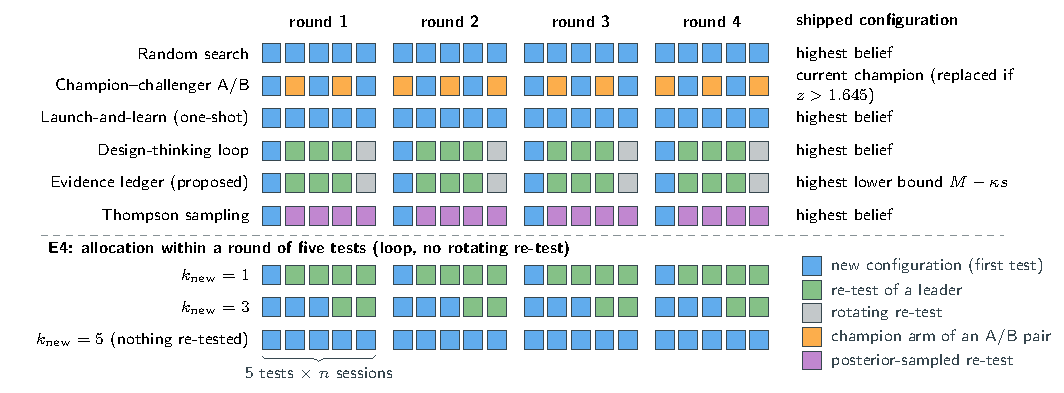
\includegraphics[width=\textwidth]{figures/fig_protocols.pdf}
\caption{Test schedules of the policies in the first four rounds (five tests per round) and the allocations varied in experiment E4. Each square is one test of $n$ sessions. Schematic drawn in TikZ with code written with the assistance of Claude (Anthropic).}
\label{fig:protocols}
\end{figure}

Ideas are variants that differ from their parent in one or two capabilities, five per round by default. The screening score of an idea has correlation $\rho$ with its true utility across the configuration space; we set $\rho=0.5$ by default, a moderately valid expert judgement, and vary it in E5.

\subsection{Experimental design and analysis}

Table~\ref{tab:experiments} summarises the nine experiments, and Figure~\ref{fig:manip} shows the manipulations of E5--E8. The primary outcome is the true utility of the configuration a policy would ship, as a percentage of $U^*$; a difference of one \emph{point} is one percent of $U^*$. Secondary outcomes are the best utility among tested configurations (\emph{found}), their difference (the \emph{cost of choosing}), the overestimation of the shipped configuration (belief minus true utility), whether the shipped configuration is a local optimum, and outcome-specific measures defined with each experiment.

\begin{table}[!tbp]
\caption{Overview of the experiments. Budgets are in tests; runs are independent simulated improvement projects.}
\label{tab:experiments}
\centering\footnotesize
\begin{tabularx}{\textwidth}{@{}P{0.75cm}P{2.45cm}LLP{1.1cm}@{}}
\toprule
Exp. & Question & Design & Outcomes & Runs\\
\midrule
E1 & Is the testbed valid? & 621 emulated experiments: emulator vs analytic model on 141 stratified configurations; noise at $n\in\{500,\ldots,4000\}$ & agreement, bias, noise ratio & 621\\
E2 & How does the loop progress? & loop and ledger, 400 tests; loop to 3,200 tests & shipped, found, believed, local optimality & 1,620\\
E3 & Which governance policy? & 6 policies $\times$ $n\in\{500,2000\}$, 400 tests & shipped, cost of choosing, overestimate & 7,200\\
E4 & New variants or re-tests? & $k_{\text{new}}\in\{\frac12,1,\ldots,5\}$ $\times$ $n\in\{500,2000,8000\}$ at 800,000 sessions & shipped & 7,200\\
E5 & What does GenAI ideation add? & $\rho\times V\times h$ full factorial, $5\times3\times3$ & shipped; partial $\eta^2$ & 9,450\\
E6 & Which biases matter? & 4 bias types $\times$ 7 levels of $b/\sigma$; favourite bias at 3 test sizes & change in shipped & 13,440\\
E7 & What if criteria move? & drift amplitude $\times$ forgetting $\gamma$; regime shift at 200 tests & tracking of current optimum & 5,400\\
E8 & Several stakeholders? & archive vs scalarised loops, 3 budgets & hypervolume, local Pareto optimality & 630\\
E9 & How robust? & 120 random scenarios $\times$ 4 policies $\times$ 12 seeds & ledger advantage; regression & 5,760\\
E10 & Review checks & stronger A/B baselines; ship-rule $\kappa$; misspecified ground truth & shipped; paired differences & 8,800\\
E11 & Audit & decomposition by design principle; misspecified noise; production start; build rate & shipped; paired differences & 17,200\\
\bottomrule
\end{tabularx}
\end{table}

\begin{figure}[!tbp]
\centering
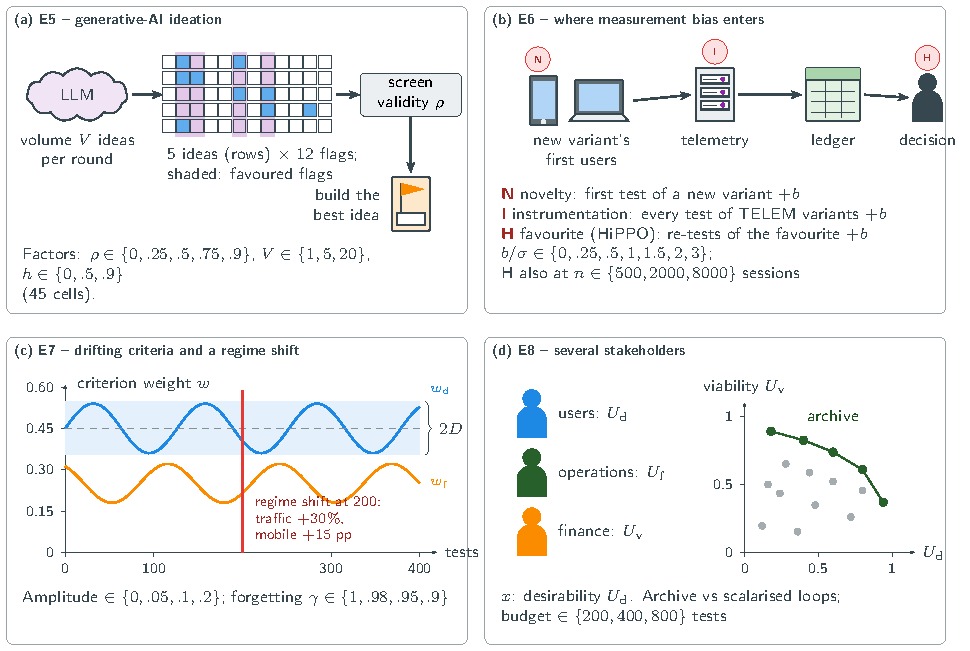
\includegraphics[width=\textwidth]{figures/fig_manip.pdf}
\caption{Manipulations of experiments E5--E8: (a) generative ideation with volume $V$, homogenisation $h$ and screening validity $\rho$; (b) the points at which novelty (N), instrumentation (I) and favourite (H) bias enter the evidence; (c) drifting criteria within a band and an abrupt regime shift; (d) stakeholders with different criteria and an archive of non-dominated variants. The weight paths in (c) and the points in (d) are illustrative, not data. Schematic drawn in TikZ with code written with the assistance of Claude (Anthropic).}
\label{fig:manip}
\end{figure}

Runs are paired by seed across conditions where possible, so that conditions share their starting configurations. On the reference instance we report means across runs with 95\% $t$-intervals; for the families we first average the runs on each instance and report means and intervals across instances, so that the instance is the unit of analysis. Paired comparisons use Wilcoxon signed-rank tests with Holm's correction within each family of comparisons, and effect sizes are reported as Cohen's $d_z$. In the factorial experiment we report partial $\eta^2$ from a balanced analysis of variance on instance-level cell means for the families and on runs for the reference instance. The numbers of runs were set so that the 95\% half-width of the main contrasts is about one point of $U^*$ on the reference instance (300 runs in E2 and E3) and so that every family instance contributes several runs; the instance-level intervals for the families are wider and are reported throughout.

% ===========================================================================
\section{Results}
\label{sec:results}

\subsection{E1: Validity of the testbed}
\label{sec:e1}

Figure~\ref{fig:e1}a compares the utility measured in one emulated experiment of 6,000 sessions with the analytic utility of 141 configurations, stratified by the utilisation of the busiest tier. For the 90 configurations below 85\% utilisation the two agree closely: the correlation is 0.85, the mean difference is 0.009 utility units, and after removing the noise of the emulated measurement ($\sigma=0.069$ at this sample size) the standard deviation of the model error is 0.044. The emulated conversion rate differs from the analytic one by 0.2\% on average, and the 95th percentile of page time correlates at 0.999 with its analytic counterpart, which it underestimates by 6\% because emulated service times are less variable than the exponential assumption of the Erlang-C formula. Near capacity (31 configurations between 85\% and 97\% utilisation) the model error grows to 0.084. Beyond capacity the two disagree sharply: in a three-minute emulated experiment the queue has not yet built up, and the emulator reports conversion 135\% higher than the steady-state model. Short online experiments thus systematically flatter configurations that operate beyond capacity, a bias we return to in Section~\ref{sec:discussion}. Configurations beyond capacity are poor under the steady-state model, and none is close to the optimum of any instance.

The noise of a test depends on its size as sampling theory predicts (Figure~\ref{fig:e1}b). Across six configurations and four sizes, the standard deviation of emulated results is on average 0.98 times that of the statistical sampler (range 0.56--1.28, with 20 replications per cell; mean log variance ratio $-0.07$, $p=0.33$), and both fall as $n^{-1/2}$, from 0.29 at 500 sessions to 0.10 at 4,000. We therefore use the analytic model as ground truth and the sampler as the test, which allows tens of thousands of runs.

\begin{figure}[!tbp]
\centering
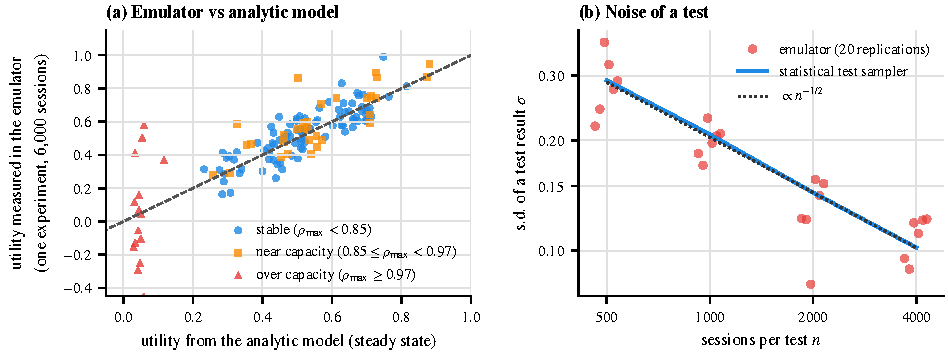
\includegraphics[width=\textwidth]{figures/fig_e1_validation.pdf}
\caption{E1: validation of the testbed. (a) Utility measured in one emulated experiment against the analytic utility for 141 configurations stratified by the utilisation of the busiest tier; the dashed line is equality. (b) Standard deviation of a test result as a function of its size: emulator (points, 20 replications for each of six configurations) and statistical sampler (line). Plotted directly from the simulation outputs with code written with the assistance of Claude (Anthropic).}
\label{fig:e1}
\end{figure}

The landscapes differ in the ways intended (Table~\ref{tab:landscapes}). The reference instance has four local optima for one-capability variants and two for variants within two capabilities; the service family has one to eight and one to three; the rugged family has three to 57 and one to 13. In every class the noise of a test of 2,000 sessions (0.05--0.20) is two to five times the spread of the fifty best configurations (0.015--0.058), so that a single test cannot separate good configurations from the best ones.

\begin{table}[!tbp]
\caption{Structure of the landscapes: medians, with ranges across instances in brackets. $\sigma(n)$ is the standard deviation of a test of $n$ sessions; ``top-50 s.d.'' is the standard deviation of the 50 best utilities.}
\label{tab:landscapes}
\centering\footnotesize
\begin{tabularx}{\textwidth}{@{}lCCC@{}}
\toprule
 & Reference (1) & Service family (30) & Rugged family (20)\\
\midrule
Optimum $U^*$ & 0.881 & 0.911 [0.871, 0.951] & 0.932 [0.876, 0.969]\\
Mean utility (s.d.) & 0.333 (0.243) & 0.345 (0.243) & 0.326 (0.212)\\
Local optima, radius 1 & 4 & 2 [1, 8] & 21 [3, 57]\\
Local optima, radius 2 & 2 & 1 [1, 3] & 5.5 [1, 13]\\
$\sigma(500)$ / $\sigma(2000)$ / $\sigma(8000)$ & 0.24 / 0.12 / 0.06 & 0.24 / 0.12 / 0.06 & 0.16 / 0.08 / 0.04\\
Top-50 s.d. & 0.032 & 0.026 [0.015, 0.055] & 0.041 [0.020, 0.058]\\
\bottomrule
\end{tabularx}
\end{table}

\FloatBarrier
\subsection{E2: The cost of choosing and the optimiser's curse (H1)}
\label{sec:e2}

On the reference instance the loop ships a configuration worth 84.1\% of the optimum after 100 tests, 89.4\% after 200 and 93.7\% after 400 (Figure~\ref{fig:e2}a). At every horizon it has already tested a better configuration: the best found is worth 87.8\%, 93.5\% and 97.4\%. After 400 tests the loop loses 2.6 points to configurations it has not found and 3.7 points to its own choice among those it has. The team's belief about the configuration it would ship exceeds that configuration's true utility by 6.1 points, so that it believes it holds 99.8\% of the optimum. The service family looks the same (losses of 2.1 and 4.1 points, overestimation 6.7 points). On the rugged family, where the best configurations differ more relative to the noise, the cost of choosing (0.8 points) and the overestimation (0.8 points) are small and finding is the larger problem (4.3 points).

\begin{figure}[!tbp]
\centering
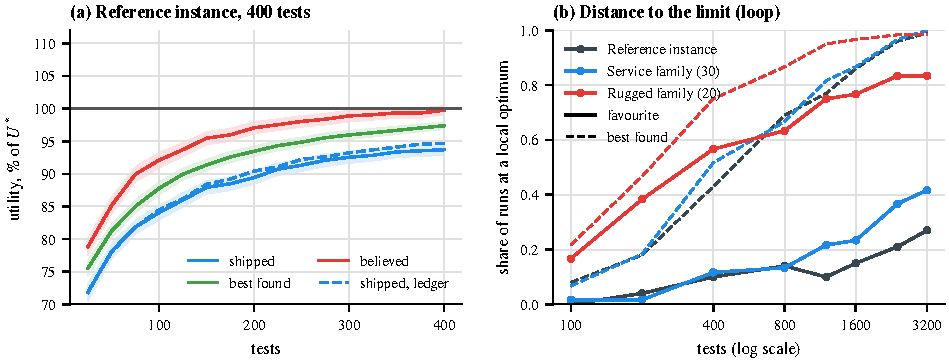
\includegraphics[width=\textwidth]{figures/fig_e2_dynamics.pdf}
\caption{E2: (a) utility shipped, best utility found and believed utility of the shipped configuration on the reference instance (300 runs; bands are 95\% confidence intervals), and the utility shipped by the evidence ledger (dashed). (b) Share of runs in which the favourite (solid) or the best tested configuration (dashed) is a local optimum (radius 2), determined by enumeration, over 3,200 tests. Plotted directly from the simulation outputs with code written with the assistance of Claude (Anthropic).}
\label{fig:e2}
\end{figure}

Discounting thin evidence (DP5) changes what is shipped, not what is found. The evidence ledger ships 94.7\% on the reference instance and 95.1\% on the service family, 1.0 and 1.3 points more than the loop (paired $p<10^{-4}$ in both; Table~\ref{tab:policies}). It reduces the cost of choosing from 3.7 to 2.7 points and from 4.1 to 2.8 points, and the overestimation from 6.1 to 4.6 and from 6.7 to 4.7 points, reductions of between a quarter and a third. On the rugged family, where little is lost by choosing, the two are equivalent. H1 is supported.

The limit of the theorem is remote (Figure~\ref{fig:e2}b). After 400 tests the favourite is a local optimum in 10\% of runs on the reference instance, 12\% on the service family and 57\% on the rugged family, although the best configuration tested already is one in 43\%, 52\% and 75\% of runs. After 3,200 tests, about eight times the budget of a typical programme, the best tested configuration is a local optimum in 98--100\% of runs while the favourite is one in only 27\%, 42\% and 83\%. As in the abstract landscapes of \citet{kuras2026}, the limiting factor at realistic horizons is recognition, not discovery.

\FloatBarrier
\subsection{E3: Experimentation-governance policies (H2)}
\label{sec:e3}

Table~\ref{tab:policies} and Figure~\ref{fig:e3} compare the six policies under 400 tests. Champion--challenger A/B testing, the most common practice, ships 84.1\%, 85.1\% and 87.1\% of the optimum with tests of 2,000 sessions, and 74.9\%, 76.7\% and 74.4\% with tests of 500, little better than random search. The evidence ledger ships 7.9 to 10.6 points more with large tests and 14.9 to 16.7 points more with small ones ($p_{\mathrm{Holm}}<10^{-4}$ on every class; $d_z$ between 0.87 and 2.4). Champion--challenger testing finds configurations as good as the ledger does (best found 96.2--98.3\%) but ships configurations 9 to 14 points worse than its own best, because each comparison is decided by one noisy test per arm and the evidence of earlier comparisons is thrown away. A single lucky test can install a poor challenger, and a single unlucky one can keep a good challenger out. Its believed utility is close to the truth only because the belief is itself one recent test result. Stronger versions of the practice do not close the gap (Section~\ref{sec:e10}): pooling the champion's evidence across experiments raises champion--challenger testing to 87.5--89.5\%, still 4.9 to 7.3 points behind the ledger ($p<10^{-3}$ on every class), and replacing the significance rule by ``ship whichever arm measured higher'' makes it worse. H2 is supported.

\begin{table}[!tbp]
\caption{E3: utility shipped after 400 tests of 2,000 sessions, as a percentage of $U^*$, with 95\% half-widths; the cost of choosing (found minus shipped) and the overestimation (believed minus shipped), in points; and the paired difference of the evidence ledger from each policy with Holm-adjusted Wilcoxon $p$ and $d_z$ (reference instance: 300 runs; families: 10 runs per instance, instance as unit).}
\label{tab:policies}
\centering\footnotesize
\setlength{\tabcolsep}{3pt}
\begin{tabular*}{\textwidth}{@{\extracolsep{\fill}}lcccccccc@{}}
\toprule
& \multicolumn{4}{c}{Reference instance} & \multicolumn{3}{c}{Service family (30)}\\
\cmidrule(lr){2-5}\cmidrule(l){6-8}
Policy & Shipped & Choose & Over & Ledger $-$ policy & Shipped & Choose & Ledger $-$ policy\\
\midrule
Random search & $83.0\pm1.2$ & 12.5 & 25.4 & $+11.6^{***}$ (0.98) & $82.8\pm1.9$ & 11.5 & $+12.3^{***}$ (2.66)\\
Champion--challenger & $84.1\pm1.2$ & 14.2 & 3.1 & $+10.6^{***}$ (0.87) & $85.1\pm1.8$ & 13.2 & $+10.1^{***}$ (2.22)\\
Launch-and-learn & $95.3\pm0.7$ & 3.9 & 6.0 & $-0.6$ ($-0.07$) & $93.6\pm1.1$ & 5.4 & $+1.5^{**}$ (0.43)\\
Design-thinking loop & $93.7\pm0.9$ & 3.7 & 6.1 & $+1.0^{***}$ (0.26) & $93.8\pm1.2$ & 4.1 & $+1.3^{***}$ (0.89)\\
Evidence ledger & $94.7\pm0.8$ & 2.7 & 4.6 & --- & $95.1\pm1.2$ & 2.8 & ---\\
Thompson sampling & $94.9\pm0.8$ & 2.4 & 4.3 & $-0.3$ ($-0.03$) & $94.8\pm1.1$ & 3.5 & $+0.3$ (0.10)\\
\bottomrule
\end{tabular*}

\smallskip
{\scriptsize $^{**}p_{\mathrm{Holm}}<0.01$; $^{***}p_{\mathrm{Holm}}<0.001$; $d_z$ in brackets. Results for the rugged family and for tests of 500 sessions are in Figure~\ref{fig:e3} and the text.\par}
\end{table}

\begin{figure}[!tbp]
\centering
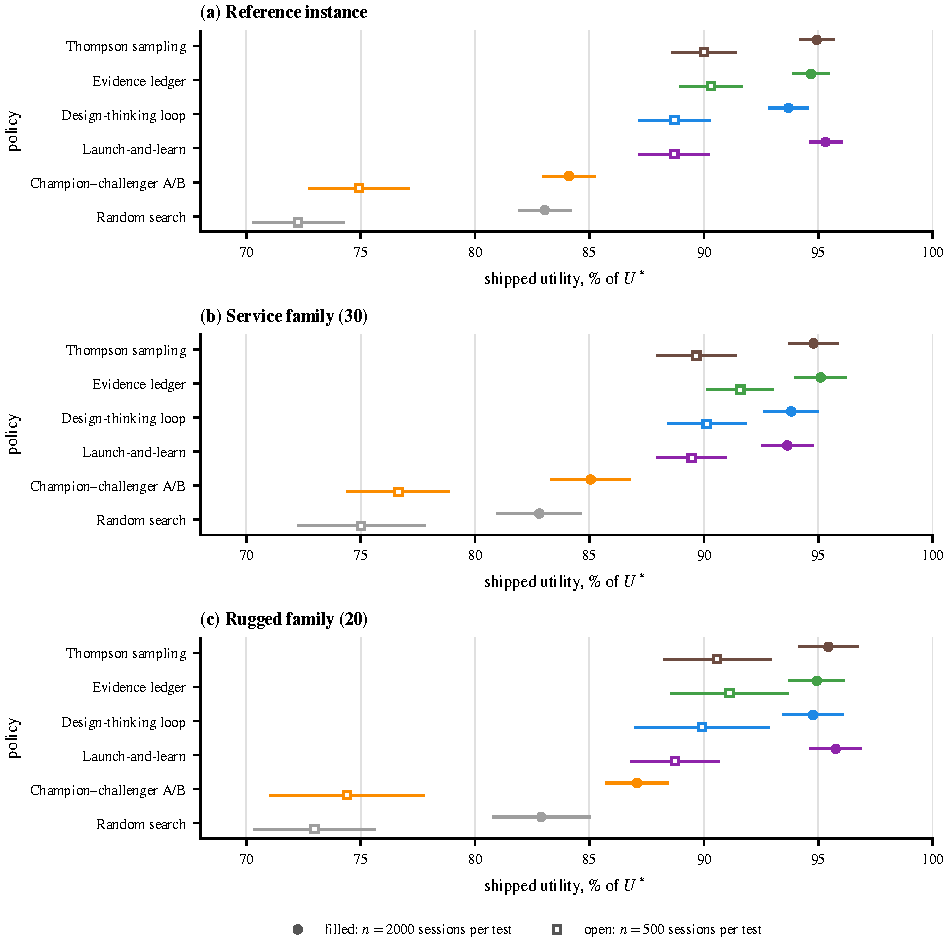
\includegraphics[width=\textwidth]{figures/fig_e3_policies.pdf}
\caption{E3: utility shipped after 400 tests by six policies, with tests of 2,000 sessions (filled) and 500 sessions (open); bars are 95\% confidence intervals (instance-level for the families). Plotted directly from the simulation outputs with code written with the assistance of Claude (Anthropic).}
\label{fig:e3}
\end{figure}

Among the policies that pool evidence the differences are an order of magnitude smaller. The ledger is level with Thompson sampling on every class and at both test sizes (differences between $-0.5$ and $+1.9$ points, none significant after correction), so that a fixed, transparent routine with a conservative ship rule does as well as a tuned bandit. Launch-and-learn, which never re-tests, is level with the ledger when tests are large (reference $-0.6$, rugged $-0.8$, both n.s.) and behind it on the service family ($-1.5$, $p_{\mathrm{Holm}}=0.008$); with small tests it is 1.6 to 2.4 points behind on all classes ($p_{\mathrm{Holm}}=0.006$ on the service family). It builds almost three times as many configurations as the ledger and finds better ones (99.2\% against 97.4\% on the reference instance), but chooses worse among them. Re-testing pays when tests are noisy.

\FloatBarrier
\subsection{E4: New variants or re-tests? (H3)}
\label{sec:e4}

Experiment E4 fixes the traffic at 800,000 sessions and varies both the size of a test and the number of new configurations built per round of five tests (Figure~\ref{fig:e4}). Two results stand out. First, building too little is the worst choice in eight of the nine combinations of class and test size: against the best allocation, a new configuration every second round costs 0.9 to 4.5 points with tests of 500 or 2,000 sessions and 8.0 to 12.6 points with tests of 8,000. Second, the best allocation is interior or near the top of the range: three or four new configurations per five tests with small and medium tests on the reference instance and the service family, and two to three on the rugged family; with the largest tests it moves to five on the two families. Spending all five tests on new configurations is never far behind the best (0.1 to 1.7 points, significant only on the service family with tests of 2,000 sessions). The optimum thus moves towards building as tests become more precise, which is the direction the theory predicts, but the penalty for building too much is much smaller than the penalty for building too little. H3 is partially supported.

\begin{figure}[!tbp]
\centering
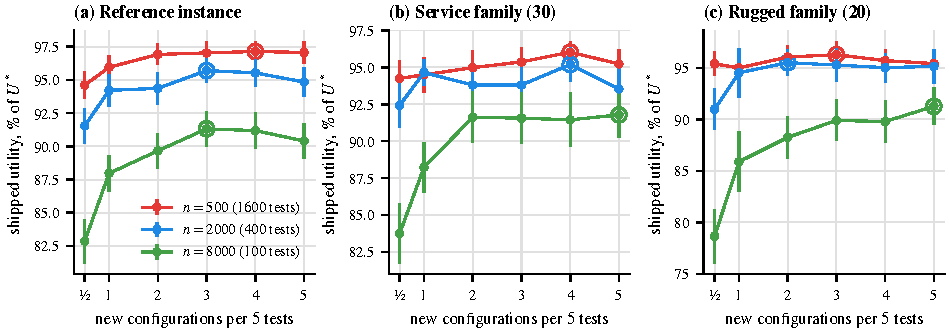
\includegraphics[width=\textwidth]{figures/fig_e4_allocation.pdf}
\caption{E4: utility shipped after 800,000 sessions as a function of the number of new configurations per five tests, for three test sizes (loop without rotating re-test; error bars are 95\% confidence intervals; circles mark the best allocation). Plotted directly from the simulation outputs with code written with the assistance of Claude (Anthropic).}
\label{fig:e4}
\end{figure}

The size of the test matters more than the allocation. Under the same traffic, many small tests beat few large ones on every class: the best allocation reaches 97.2\%, 96.0\% and 96.3\% of the optimum with 1,600 tests of 500 sessions, 95.7\%, 95.2\% and 95.5\% with 400 tests of 2,000, and 91.3\%, 91.8\% and 91.3\% with 100 tests of 8,000. More, smaller tests mean more rounds of the loop, and the ledger can concentrate repeated small tests on the leaders where a single large test would spread precision over a variant that turns out to be poor. The result parallels the analysis of \citet{azevedo2020}, who show that many smaller experiments are preferable when the distribution of improvements has fat tails; in our setting the same conclusion follows from the ability to re-test.

\FloatBarrier
\subsection{E5: Generative ideation (H4)}
\label{sec:e5}

Experiment E5 crosses the validity of screening ($\rho$), the number of ideas proposed per round ($V$) and their homogenisation ($h$, the share of ideas whose changes are confined to four favoured capabilities; Figure~\ref{fig:manip}a). Figure~\ref{fig:e5} shows the main result. Without valid screening, more ideas are worth nothing: with $\rho=0$, twenty ideas per round ship the same utility as one (differences of $+0.1$, $0.0$ and $-1.2$ points; all n.s.), because the team has no way to tell which of them to build. This part of the result is a structural property of the model, in which ideas are exchangeable unless a screen distinguishes them, rather than an empirical finding; the empirical content lies in the size of the effect of validity and in its interaction with volume and homogenisation. With valid screening, the gains are large: raising $\rho$ from 0 to 0.9 adds 4.8, 3.4 and 7.2 points on average over the cells with five or twenty ideas. Moving from five to twenty ideas adds 2.0, 1.0 and 2.4 points. In an analysis of variance restricted to $V\in\{5,20\}$ (instance-level cell means for the families, runs for the reference instance), validity explains more variance than volume on every class (partial $\eta^2$ of 0.058 against 0.021 on the reference instance, 0.096 against 0.015 on the service family and 0.254 against 0.066 on the rugged family; Table~\ref{tab:eta}). H4 is supported.

\begin{figure}[!tbp]
\centering
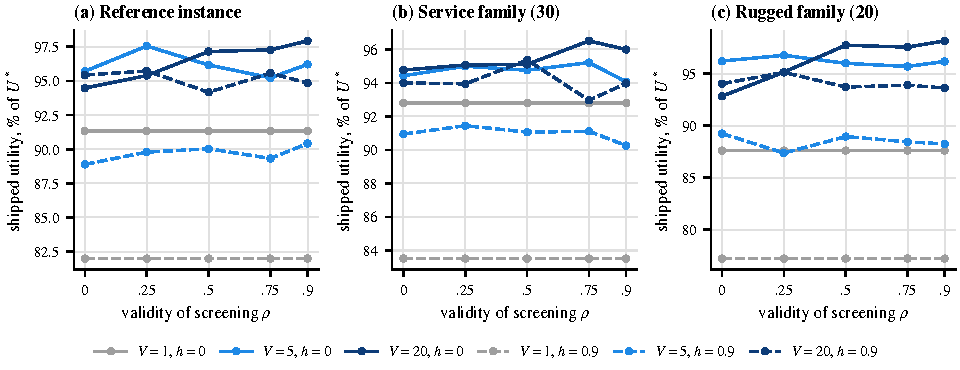
\includegraphics[width=\textwidth]{figures/fig_e5_genai.pdf}
\caption{E5: utility shipped after 400 tests by the evidence ledger as a function of the validity of screening $\rho$, for one, five and twenty ideas per round ($V$) and without ($h=0$, solid) or with strong homogenisation of ideas ($h=0.9$, dashed). Plotted directly from the simulation outputs with code written with the assistance of Claude (Anthropic).}
\label{fig:e5}
\end{figure}

\begin{table}[!tbp]
\caption{E5: partial $\eta^2$ of the factors of generative ideation for shipped utility, from a balanced analysis of variance restricted to five and twenty ideas per round (instance-level cell means for the families; runs for the reference instance).}
\label{tab:eta}
\centering\footnotesize
\begin{tabularx}{0.8\textwidth}{@{}lCCC@{}}
\toprule
Effect & Reference & Service family & Rugged family\\
\midrule
Validity of screening $\rho$ & 0.058 & 0.096 & 0.254\\
Volume $V$ & 0.021 & 0.015 & 0.066\\
Homogenisation $h$ & 0.048 & 0.048 & 0.150\\
$\rho\times V$ & 0.004 & 0.002 & 0.024\\
$\rho\times h$ & 0.003 & 0.011 & 0.020\\
$V\times h$ & 0.005 & 0.005 & 0.043\\
\bottomrule
\end{tabularx}
\end{table}

Homogenisation is costly. Confining 90\% of ideas to a few favoured capabilities costs 5.8, 4.7 and 6.1 points on average across cells and, with a single idea per round, about ten points on every class, because the loop can no longer reach the capabilities that matter. Volume partly compensates: with twenty homogenised ideas a valid screen still finds the occasional idea outside the favoured set. A language model that generates many similar ideas, in the manner reported by \citet{doshi2024}, is therefore worth much less than its volume suggests, and its value rests on the quality of the judgement that selects among its ideas.

\FloatBarrier
\subsection{E6: Measurement bias (H5)}
\label{sec:e6}

Figure~\ref{fig:e6}a shows the change in shipped utility when one of three biases is injected into the tests (Figure~\ref{fig:manip}b), relative to the same runs without bias. A bias that inflates every re-test of the current favourite, the signature of the highest paid person's opinion or of confirmation-seeking analysis, has no detectable effect up to half the standard deviation of a test; at $b=\sigma$ it costs 1.1 to 2.3 points, at $2\sigma$ 3.1 to 5.7 and at $3\sigma$ 6.2 to 11.6. A novelty effect that inflates the first test of every new variant is harmless up to $2\sigma$ and costs at most 2.6 points at $3\sigma$, because the re-tests of the leaders correct it. An instrumentation bias that inflates every test of configurations with fine-grained telemetry, for example because better tracking captures conversions that other configurations miss, is harmless up to about $\sigma$ but then grows fastest of all: $-2.1$ to $-5.8$ points at $2\sigma$ and $-6.2$ to $-14.9$ at $3\sigma$. Re-testing cannot remove it, since every test of an affected configuration is biased in the same direction. An audit of ten tests that estimates the bias by comparing instrumented with server-side measurements, and corrects subsequent tests, caps the loss at 0.3 to 0.9 points (n.s.) at every level of bias, including the audit's own cost.

\begin{figure}[!tbp]
\centering
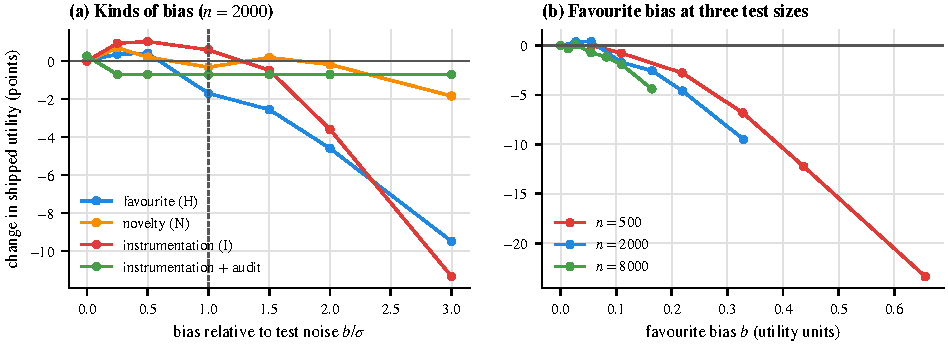
\includegraphics[width=\textwidth]{figures/fig_e6_bias.pdf}
\caption{E6: change in shipped utility after 400 tests relative to unbiased runs (mean over the three landscape classes). (a) Favourite, novelty and instrumentation bias as multiples of the test noise $\sigma$, and instrumentation bias with an audit of ten tests. (b) Favourite bias in absolute utility units for three test sizes. Plotted directly from the simulation outputs with code written with the assistance of Claude (Anthropic).}
\label{fig:e6}
\end{figure}

The threshold scales with the noise of a test (Figure~\ref{fig:e6}b). A favourite bias of 0.11 utility units costs 1.4 to 2.2 points with precise tests of 8,000 sessions, where it equals $2\sigma$, but at most 1.2 points with tests of 500 sessions, where it equals $\sigma/2$. Precise measurement makes an experimentation programme more, not less, vulnerable to its own bias. H5 is supported.

\FloatBarrier
\subsection{E7: Drifting criteria and regime shifts (H6)}
\label{sec:e7}

When the weights of the three criteria oscillate during the programme (Figure~\ref{fig:manip}c), the loop keeps tracking the moving optimum (Figure~\ref{fig:e7}a). Averaged over tests 100 to 400, the shipped configuration is worth 90.4--91.9\% of the current optimum without drift and 89.3--91.3\% with the largest amplitude, which moves the utility of configurations by a median $D=0.14$. Corollary T3 is satisfied with room to spare: at 400 tests the best variant of the shipped configuration beats it by a median 0.015 to 0.019 under the current criteria, within $4D$ in 93\% of runs at the smallest amplitude and in all runs at the largest. Forgetting old evidence makes no material difference under drift: the means for the four forgetting factors differ by at most 1.4 points, within their confidence intervals.

\begin{figure}[!tbp]
\centering
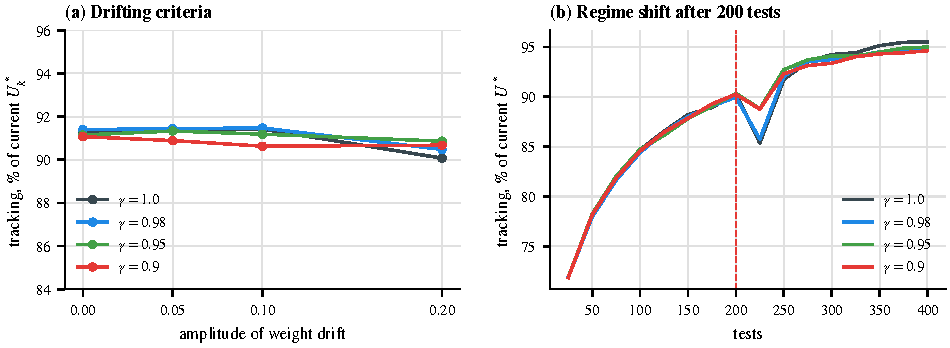
\includegraphics[width=\textwidth]{figures/fig_e7_drift.pdf}
\caption{E7: (a) mean tracking of the current optimum between 100 and 400 tests as a function of the amplitude of drift in the criterion weights, for four forgetting factors $\gamma$; (b) tracking before and after a regime shift at 200 tests (traffic $+30\%$, mobile share $+15$ percentage points), mean over the three classes. Plotted directly from the simulation outputs with code written with the assistance of Claude (Anthropic).}
\label{fig:e7}
\end{figure}

An abrupt shift is different (Figure~\ref{fig:e7}b). When traffic rises by 30\% and the mobile share by 15 percentage points after 200 tests, capacity-hungry configurations lose value, and the configuration the ledger would ship drops from 90.3\% to 85.4\% of the new optimum. With forgetting at $\gamma=0.95$ the drop is to 88.8\%; on the reference instance this is 7.7 points better 25 tests after the shift ($p=0.02$). The advantage disappears within 50 tests, and by 400 tests strong forgetting ($\gamma=0.9$) is 2.0 points worse on the rugged family ($p=0.01$), because it discards evidence the loop still needs. H6 is supported for bounded drift and only partly for forgetting: forgetting buys a faster first response to a shift at the price of a slightly worse long-run choice, which argues for forgetting that is triggered by a detected shift rather than applied continuously \citep{gama2014, garivier2011}.

\FloatBarrier
\subsection{E8: Several stakeholders (H7)}
\label{sec:e8}

In E8 users, operations and finance each care about one criterion (Figure~\ref{fig:manip}d). The true Pareto front contains 41 configurations on the reference instance, 17--72 on the service family and 6--26 on the rugged family. We compare the ledger with a Pareto archive, three loops that split the budget and each optimise a different weighting (0.6 on one criterion, 0.2 on the others), and a single loop with the default weights. Coverage is measured by the hypervolume of the true criteria of the delivered configurations as a share of that of the true front \citep{zitzler1999}.

\begin{figure}[!tbp]
\centering
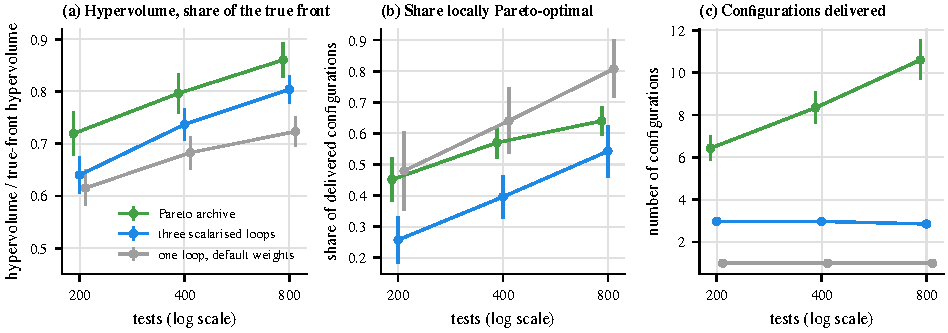
\includegraphics[width=\textwidth]{figures/fig_e8_pareto.pdf}
\caption{E8: (a) hypervolume of the delivered configurations as a share of the hypervolume of the true Pareto front, (b) share of delivered configurations that no variant within two capabilities dominates, and (c) number of configurations delivered, for a Pareto archive, three scalarised loops sharing the budget and one loop with fixed weights (means over the three classes; bars are 95\% confidence intervals). Plotted directly from the simulation outputs with code written with the assistance of Claude (Anthropic).}
\label{fig:e8}
\end{figure}

The archive covers the front better at every budget (Figure~\ref{fig:e8}a): its hypervolume share is 0.67--0.75 after 200 tests and 0.82--0.88 after 800, against 0.57--0.68 and 0.76--0.85 for the scalarised loops. The paired advantage of 0.03 to 0.09 is significant in eight of the nine combinations of class and budget. By 400 tests half or more of the archive's members are locally Pareto-optimal (0.50, 0.50 and 0.72 on the three classes), against 0.32, 0.32 and 0.54 of the configurations delivered by the scalarised loops, and the archive offers the decision makers six to twelve mutually incomparable configurations instead of three. The single configuration shipped by a loop with fixed weights is more often locally Pareto-optimal, because the whole budget serves one trade-off, but it represents only that trade-off. H7 is supported: when stakeholders have not agreed on weights, an archive defers the disagreement without wasting tests on it.

\FloatBarrier
\subsection{E9: Robustness (H8)}
\label{sec:e9}

Experiment E9 draws 120 scenarios at random: the landscape family and instance, the number of capabilities (10, 12 or 14, that is 1,024 to 16,384 configurations), the size of a test (400 to 8,000 sessions), the budget (100 to 800 tests), the validity of screening (0.2 to 0.8), the number of ideas per round (2 to 15) and the reach of ideation (variants within one, two or three capabilities). In each scenario four policies run twelve times with common seeds. The resulting signal-to-noise ratios, the spread of the fifty best utilities divided by the noise of a test, range from 0.07 to 2.1.

The ledger ships a better configuration than champion--challenger testing in 90\% of the scenarios, by 7.6 points on average (median 6.0; tenth percentile 0.3, ninetieth 17.1). Figure~\ref{fig:e9}a shows how the advantage depends on the scenario in a regression on standardised factors with heteroscedasticity-robust intervals ($R^2=0.69$). The advantage is larger when the signal-to-noise ratio is low ($-3.4\pm1.4$ points per standard deviation of its logarithm), when the budget is larger ($+3.2\pm0.8$), because champion--challenger testing cannot accumulate evidence however long it runs, and when tests are small ($-2.1\pm1.1$ per standard deviation of log test size); the reach of ideation and the number of ideas make no difference to it. Against launch-and-learn the ledger is ahead by 1.1 points on average ($\pm0.7$) and in 63\% of scenarios, more so when screening is valid ($+1.4\pm0.7$) and when the signal-to-noise ratio is low ($-2.0\pm1.4$); against the plain loop it is ahead by $0.3\pm0.2$ points, the gain of its ship rule, which grows with the budget. H8 is supported.

\begin{figure}[!tbp]
\centering
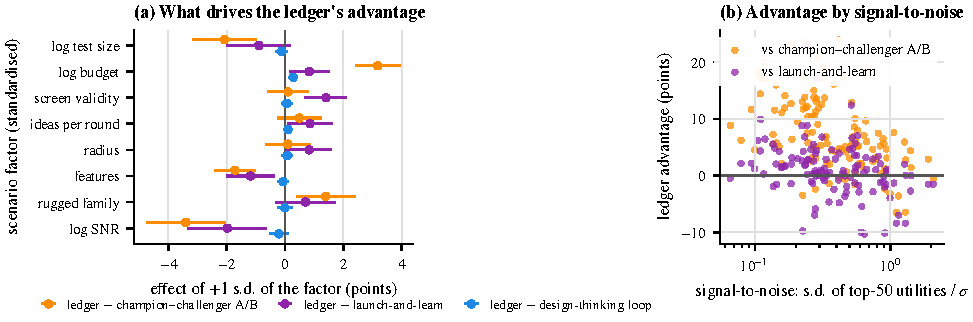
\includegraphics[width=\textwidth]{figures/fig_e9_robustness.pdf}
\caption{E9: (a) coefficients of a regression of the ledger's advantage over three policies on standardised scenario factors (120 scenarios, 12 runs each; bars are 95\% heteroscedasticity-robust intervals); (b) the advantage over champion--challenger and launch-and-learn against the signal-to-noise ratio of the scenario. Plotted directly from the simulation outputs with code written with the assistance of Claude (Anthropic).}
\label{fig:e9}
\end{figure}

\FloatBarrier
\subsection{E10: Robustness checks requested in review}
\label{sec:e10}

Three checks address the strongest objections to the evaluation (Table~\ref{tab:e10}; 150 runs on the reference instance and five per family instance, tests of 2,000 sessions, 400 tests). First, the practice baseline was strengthened. Pooling the champion's evidence over all the experiments in which it took part raises champion--challenger testing by three to four points; letting the higher-measuring arm win without a significance test lowers it by eight to thirteen points, because single noisy comparisons then replace the champion at random. The ledger leads the strongest variant by 7.3, 6.5 and 4.9 points ($p\le0.0003$). Second, the constant $\kappa$ of the ship rule, which was set to one posterior standard deviation a priori and not tuned, matters little between 0.5 and 2 (differences within 0.8 points on every class); $\kappa=0$ is the plain loop. Third, the ground truth was perturbed: every configuration's true utility was shifted by a fixed random error with the standard deviation of the model error measured in E1 (0.044) or twice that, so that the testbed's model is wrong in the way and by the amount the emulation suggests. The ledger's lead over champion--challenger testing remains between 5.5 and 11.8 points; its lead over the plain loop shrinks to 0.0--0.5 points, and launch-and-learn remains level with it.

\begin{table}[!tbp]
\caption{E10: utility shipped after 400 tests (\% of $U^*$; reference instance and means over family instances) under stronger practice baselines, different ship-rule constants and a misspecified ground truth with error s.d. $\tau$.}
\label{tab:e10}
\centering\footnotesize
\begin{tabularx}{\textwidth}{@{}P{7.4cm}CCC@{}}
\toprule
Condition & Reference & Service family & Rugged family\\
\midrule
\multicolumn{4}{@{}l}{\textit{(a) Practice baselines and the ledger}}\\
Champion--challenger, 5\%, evidence not pooled & 84.0 & 84.9 & 86.8\\
Champion--challenger, 5\%, champion's evidence pooled & 87.5 & 88.3 & 89.5\\
Champion--challenger, ship the higher arm, pooled & 79.9 & 79.8 & 83.5\\
Evidence ledger ($\kappa=1$) & 94.8 & 94.8 & 94.4\\
\addlinespace[3pt]
\multicolumn{4}{@{}l}{\textit{(b) Ship-rule constant of the ledger}}\\
$\kappa=0$ (the plain loop) & 94.0 & 93.7 & 94.6\\
$\kappa=0.5$ & 94.5 & 94.3 & 94.6\\
$\kappa=1.5$ & 95.0 & 95.1 & 94.4\\
$\kappa=2$ & 95.0 & 95.0 & 94.4\\
\addlinespace[3pt]
\multicolumn{4}{@{}l}{\textit{(c) Misspecified ground truth: paired difference of the ledger, points}}\\
vs champion--challenger, $\tau=0.044$ & $+9.9$ & $+11.8$ & $+6.1$\\
vs champion--challenger, $\tau=0.088$ & $+7.4$ & $+8.6$ & $+5.5$\\
vs loop, $\tau=0.044$ & $+0.5$ & $+0.4$ & $+0.4$\\
vs loop, $\tau=0.088$ & $+0.5$ & $0.0$ & $+0.1$\\
\bottomrule
\end{tabularx}
\end{table}

\FloatBarrier
\subsection{E11: Audit of the evaluation}
\label{sec:e11}

A final set of experiments audits the evaluation itself (Figure~\ref{fig:e11}; 150 runs on the reference instance and five per family instance, 400 tests of 2,000 sessions). The audit also found a defect in the champion--challenger implementation: when every variant of the champion had been built, which happened in runs with a small ideation reach, the policy stopped experimenting before its budget was spent. It was corrected to propose variants of another tested configuration, and E3, E9 and E10 were re-run; the correction raised the champion--challenger results by up to three points on the rugged family and removed an apparent effect of ideation reach in E9. All numbers reported above are from the corrected runs.

\emph{Decomposition by design principle.} Figure~\ref{fig:e11}a adds the ledger's elements to champion--challenger testing one at a time. Pooling the champion's evidence across experiments is worth 3.5, 3.4 and 2.7 points on the three classes ($p\le0.03$). Retaining every tested variant and shipping the best pooled belief adds 1.2, 0.6 and $-0.5$ points (n.s.); screening the idea pool as the loop does, rather than the current round's ideas, adds nothing ($-0.1$, $-1.1$ and $-2.3$, n.s.), so the ledger's advantage does not come from a better use of the screen. Re-testing the favourite four times per build instead of once adds 4.0, 4.5 and 2.8 points ($p\le0.014$), and re-testing three leaders instead of one 1.6, 1.2 and 2.7 (significant only on the rugged family). The rotating re-test, which the theorem's fourth assumption requires, adds $-0.2$, $-1.0$ and $0.0$ points within 400 tests, and the ship rule 0.8, 1.1 and $-0.1$. The practices that matter at this horizon are therefore pooling evidence across experiments and giving each new variant several tests before deciding about it; the rotation that guarantees convergence in the limit has no value in a programme of this length.

\emph{Misspecified test noise.} The beliefs assume the noise of a test to be the landscape average, but the noise is larger for better configurations (its standard deviation is 0.156 among the fifty best configurations of the reference instance against 0.120 on average, with a correlation of 0.88 between noise and utility). Assuming a noise 30\% larger than the average, which is what the leaders have, changes shipped utility by $+0.3$ to $+1.4$ points for the ledger, the loop and launch-and-learn; assuming half the true noise costs 0.0 to 0.6 points and assuming twice the true noise 1.0 to 1.5. Estimating the noise online from the re-test residuals of the ledger's own variants, which converges to about 0.145 on the reference instance, changes nothing ($-0.5$ to $0.0$, n.s.). The results are therefore insensitive to the homoscedasticity assumption within the range that the testbed exhibits.

\emph{Starting point and build rate.} The experiments above start a programme from five random configurations, which are worth 38\% of the optimum on average; a real programme starts from the configuration in production, with evidence from its history. Starting from the bare service (57\% of the optimum, with ten free tests of history) and four screened one-capability variants lowers every policy's result, by 0.2 to 1.9 points for champion--challenger testing and launch-and-learn and by 0.8 to 3.0 points for the ledger with its default of one build per five tests (Figure~\ref{fig:e11}b). From such a start the ledger builds too little: raising its build rate to three per five tests recovers 5.6, 0.9 and 1.7 points ($p<10^{-7}$ on the reference instance), so that the ledger is again level with launch-and-learn ($-0.1$, $+0.8$ and $+0.2$, n.s.) and 5.8 to 8.5 points ahead of pooled champion--challenger testing ($p<10^{-4}$). With a random start the build rate matters less ($+1.4$, $-0.7$ and $+0.6$ for three builds against one). The default build rate of the ledger, inherited from the design-thinking loop and from the theorem's emphasis on re-testing, was thus too conservative for a realistic programme, and the recommendation in Section~\ref{sec:discussion} is adjusted accordingly.

\begin{figure}[!htbp]
\centering
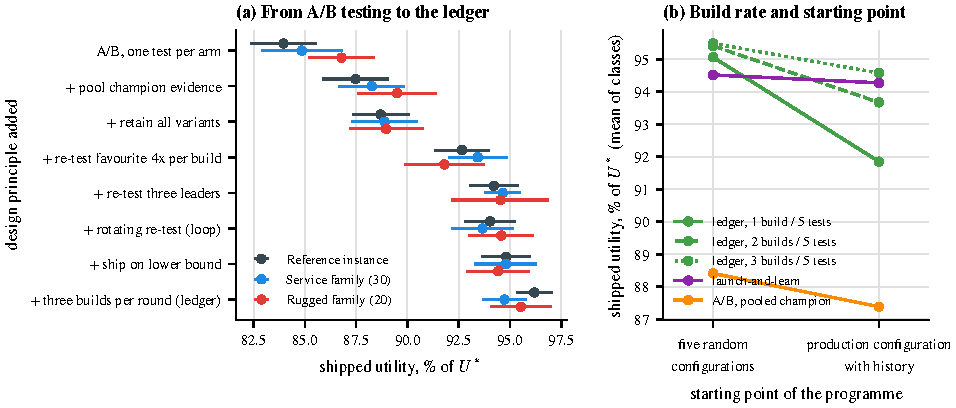
\includegraphics[width=\textwidth]{figures/fig_e11_audit.pdf}
\caption{E11: (a) utility shipped after 400 tests as the ledger's elements are added one at a time to champion--challenger testing (bars are 95\% confidence intervals; instance-level for the families); (b) utility shipped by five policies from a random start and from the production configuration with history, mean over the three landscape classes. Plotted directly from the simulation outputs with code written with the assistance of Claude (Anthropic).}
\label{fig:e11}
\end{figure}
\FloatBarrier


% ===========================================================================
\section{Discussion}
\label{sec:discussion}

\subsection{Summary of findings}

Table~\ref{tab:hyp} summarises the evidence. Six hypotheses are supported and two partly. The convergence theorem of \citet{kuras2026} survives the move from abstract landscapes to a digital service whose utility emerges from capacity, latency, conversion and cost, and whose test noise is set by traffic. Its conditions translate into design principles whose violation is costly, and the finite-horizon findings it reports, namely a remote limit, a large cost of choosing, an optimiser's curse, a bias threshold near the noise level and the importance of screening, reappear in the testbed with similar magnitudes. Two of its finite-horizon results do not carry over unchanged. Spending every test on new configurations is not the worst allocation in a digital service with valid screening and many small tests: it is close to the best, and too little building is the costly error. And forgetting, which the drift corollary might seem to recommend, is of little value under bounded drift and of transient value after a shift. The decomposition of the ledger's advantage is also instructive (E11): pooling the champion's evidence and re-testing more often per build contribute about three and four points each, re-testing three leaders instead of one about one to three, discounting thin evidence when shipping about one, and the rotating re-test that the theorem's fourth assumption calls for nothing at all within 400 tests; the increment of the ship rule shrinks when the model of the service is itself uncertain (E10).

\begin{table}[!tbp]
\caption{Hypotheses and evidence.}
\label{tab:hyp}
\centering\footnotesize
\begin{tabularx}{\textwidth}{@{}P{2.6cm}LP{1.55cm}@{}}
\toprule
Hypothesis & Evidence & Verdict\\
\midrule
H1 choosing & loop loses 3.7--4.1 points to its own choice and overrates it by 6.1--6.7 points on smooth landscapes; ship rule of DP5 cuts both by a quarter to a third (E2) & supported\\
H2 governance & ledger beats champion--challenger by 7.9--16.7 points under equal traffic on every class, and its strongest pooled variant by 4.9--7.3 points (E3, E10) & supported\\
H3 allocation & optimum interior or near all-new; moves towards building as tests get precise; building too little costs most (E4) & partly\\
H4 GenAI & with $\geq5$ ideas, validity of screening explains 3--6 times more variance than volume; volume without validity adds nothing; homogenisation costs 5--6 points (E5) & supported\\
H5 bias & favourite and novelty bias harmless below $\sigma$; instrumentation bias grows fastest, survives re-testing, is neutralised by an audit (E6) & supported\\
H6 drift & bounded drift costs about one point and stays within $4D$; forgetting helps only in the first tests after a shift (E7) & partly\\
H7 stakeholders & archive covers 0.03--0.09 more of the true front's hypervolume than scalarised loops (E8) & supported\\
H8 robustness & ledger beats champion--challenger in 90\% of 120 random scenarios (mean $+7.6$ points); advantage grows as signal-to-noise falls (E9) and survives a misspecified ground truth (E10) & supported\\
\bottomrule
\end{tabularx}
\end{table}

\subsection{Implications for research}

\emph{Evaluation as the scarce resource.} Information management research has examined how organisations acquire analytics capabilities and how data-driven decisions create value \citep{gupta2016, mikalef2021, brynjolfsson2016}. Our results locate a specific and large source of value inside the experimentation capability: the management of evidence across a sequence of experiments. In every class the configurations found by different policies differ by a few points, whereas the configurations shipped differ by up to seventeen, and the difference is made by retaining, pooling, re-testing and discounting evidence. Champion--challenger testing, which treats each experiment as a self-contained decision, wastes most of what its experiments reveal. This suggests a shift of attention, in research on experimentation and data-driven decision making, from the quality of single experiments \citep{kohavi2020, fabijan2019} to the evidence architecture of experimentation programmes.

\emph{Kernel theory for experimentation systems.} The study contributes a design theory in the sense of \citet{gregor2007}: eight principles with a stated purpose, a kernel theory that explains why they work, an instantiation and an evaluation. The kernel theory adds something that experimentation practice lacks, namely a statement of the conditions under which a sequence of experiments must improve the outcome and of what each violation costs. It also shows where the bandit literature \citep{russo2018, scott2015} and the experimentation literature meet. A transparent loop that retains, re-tests and discounts does as well as Thompson sampling, so that organisations need not adopt adaptive algorithms they cannot audit in order to manage evidence well.

\emph{Generative AI shifts the bottleneck.} Research on generative AI in organisations has emphasised productivity and creativity in generation \citep{noy2023, dellacqua2023, girotra2023, boussioux2024, dwivedi2023}. \citet{girotra2023} conjectured that, once language models make ideas cheap, the bottleneck of innovation moves to evaluation and selection, and \citet{si2025} found that language-model ideas judged more novel than experts' came with unreliable self-evaluation and low diversity. Our results support the conjecture and quantify it: within an iterative improvement process, generation is valuable only through the evaluation it feeds. Without a valid screen, twenty ideas are worth no more than one; with one, the validity of the screen matters three to six times more than the number of ideas, and homogenised ideas, which several studies observe in language-model output \citep{doshi2024, anderson2024, meincke2024}, lose much of their value. The construct that IS research should measure in AI-assisted innovation is therefore the validity of AI-assisted judgement, for example of language models used as judges \citep{zheng2023}, together with the diversity of the ideas they produce, rather than the volume of output. This reframes a question raised in the IJIM debate on generative AI \citep{dwivedi2023}, namely where its value in knowledge work lies, for the setting of continuous product improvement.

\emph{A typology of measurement bias.} The bias results distinguish transient biases, which re-testing corrects and which are harmless below the noise of a test, from persistent biases attached to the measurement of particular configurations, which re-testing cannot correct. The threshold of harm scales with test noise, so that more precise measurement makes an experimentation programme more sensitive to its own bias. For research on data quality in analytics, which has long treated accuracy as one dimension among several \citep{wang1996}, this implies that the materiality of a bias depends on the precision of the measurement system it contaminates, and on whether it is attached to the alternatives being compared. A further persistent bias appeared in validation: short experiments flatter configurations that run beyond capacity, because queues take longer to build than the experiment lasts.

\emph{Methodology.} The testbed itself is a contribution: a validated, programmable environment in which the true value of every alternative is known, which allows experimentation systems to be compared on outcomes that field data cannot reveal. It follows the advice of \citet{davis2007} to use simulation where processes are path dependent and outcomes hard to observe, and the call of \citet{venable2016} to evaluate artefacts artificially before naturalistic evaluation.

\subsection{Implications for practice}

Seven recommendations follow for managers of digital services and of experimentation platforms.

\begin{enumerate}[leftmargin=*,itemsep=2pt]
\item \emph{Replace champion--challenger sequences with an evidence ledger.} Keep every tested variant, pool its results across experiments, and re-test the leaders. Under the same traffic this was worth 7.9 to 16.7 points of the attainable utility in our testbed.
\item \emph{Do not ship the apparent winner at face value.} Rank candidates by a lower confidence bound and expect the chosen variant's measured lift to shrink after launch; in our testbed the winner was overrated by 5 to 7 percent of the optimum even after 400 tests.
\item \emph{Run many small tests rather than few large ones, and keep building.} Under a fixed traffic budget, 1,600 tests of 500 sessions beat 100 tests of 8,000 by five points, and building a new variant less than once per round was the costliest allocation. A programme that starts from the production configuration should build two or three new variants per five tests and spend the rest on re-tests of the leaders (E11); one build per five tests, the rate inherited from the design-thinking loop, costs up to five points from such a start. Tests must nevertheless stay large enough for metrics to be stable and for sample-ratio checks to have power \citep{fabijan2019}.
\item \emph{Invest in screening before investing in generation.} Before scaling generative ideation, validate the judgement that selects among ideas, and monitor the diversity of the ideas. The ledger makes validation cheap: the correlation between the screening scores of built ideas and their first test results, corrected for the reliability of a single test, estimates the validity of the screen, and it can be compared across a model, a panel and their combination.
\item \emph{Audit persistent measurement bias.} Novelty effects and enthusiasm for the incumbent are tolerable if smaller than the noise of a test, but biases tied to how particular variants are measured, such as differential tracking or instrumentation, must be estimated, for example by A/A comparisons with server-side measurement, and corrected.
\item \emph{Test capacity-sensitive changes with capacity models.} Short online experiments understate the cost of configurations that overload a tier; combine them with load tests or queueing estimates.
\item \emph{Keep trade-offs open when stakeholders disagree, and forget only after shifts.} An archive of non-dominated variants represents disagreeing stakeholders better than an early compromise on weights, and old evidence should be discounted when a shift is detected, not continuously.
\end{enumerate}

Experimentation on users also raises ethical and regulatory questions that an experimentation information system should help manage rather than hide: users exposed to variants should be covered by the service's consent and privacy terms, variants that change prices, authentication or data collection deserve review before exposure, and the ledger's record of who saw what, when and with which result supports accountability. Several principles here, notably auditing measurement and re-testing before shipping, reduce the number of users exposed to variants that a single lucky test would otherwise have promoted.

\subsection{Limitations and future research}

The study evaluates the artefact in an artificial setting. The testbed is grounded in queueing theory and validated against a discrete-event emulation, but it is not a real service: its parameters are plausible rather than estimated, the emulation shares the model's structural assumptions (exponential service times, Poisson arrivals and a simple behavioural model of conversion), and both depart from the analytic model near and beyond capacity. The magnitudes we report are therefore properties of the testbed, and the qualitative patterns are what we expect to generalise; E9 shows how far they hold across a wide range of settings, and E11 shows that the artefact's own defaults, chosen from the theory rather than tuned, are not the best ones for a programme that starts from a running service. A naturalistic evaluation on a real experimentation platform, for example by replaying logged experiments through the ledger or by a field experiment that assigns product teams to governance policies, is the natural next step.

The model of a test is simplified. A real experiment returns reasons as well as numbers, which direct the next idea; it uses a concurrent control group, which removes common shocks; and its users may be exposed to several variants. Concurrent controls and variance reduction \citep{deng2013} would reduce the noise of comparisons and could change the best allocation. Common shocks, such as day-of-week effects or a marketing campaign, are absent from our tests; they make results obtained at different times less comparable, which would penalise all policies that compare a new variant with evidence collected earlier, the ledger included, and favour designs that re-test leaders concurrently with challengers. Building a variant is also free in our model, apart from its tests; where engineering effort makes building dearer than testing, the best allocation moves towards re-testing, which strengthens the case for the ledger relative to launch-and-learn. Our screening model represents judgement by a single validity coefficient, while the validity of real judges varies with the region of the space and may be correlated with the generator's own biases. The configuration space has 1,024 to 16,384 members; very large spaces of continuous parameters call for correlated beliefs and model-based optimisation \citep{frazier2008}. Finally, we hold the frame of the problem fixed within a programme; how organisations decide to reframe, which \citet{kuras2026} treat only briefly and which is central to design thinking \citep{dorst2011}, is outside our scope.

% ===========================================================================
\section{Conclusion}
\label{sec:conclusion}

Iterative online experimentation is how digital services improve, and generative AI is making its first step almost free. We asked how an experimentation information system should manage the evidence that such a process produces. A convergence theorem for the iterate--test loop gave eight design principles, an evidence ledger instantiated them, and a validated testbed with more than fifty thousand simulated improvement projects evaluated them. Retaining and pooling evidence, re-testing leaders, discounting thin evidence, auditing persistent bias and keeping stakeholder trade-offs open each have measurable value, and together they ship configurations far better than the champion--challenger practice that dominates industry. The value of generative ideation depends on the validity of the judgement that screens it more than on its volume. As ideas become cheap, the scarce resource in an experimentation programme is evaluation, and managing it is a task for information management.

% ===========================================================================
\section*{Data availability}
\ifanon
The code of the testbed, the scripts that produce every figure, table and number, and the raw outputs are deposited in a public repository \citep{dataset2026}; its identifier is withheld for anonymous review. All experiments use fixed random seeds.
\else
The code of the testbed, the scripts that produce every figure, table and number, and the raw outputs are openly available in a public repository \citep{dataset2026}. All experiments use fixed random seeds and require Python with \texttt{numpy}, \texttt{scipy}, \texttt{simpy} and \texttt{matplotlib}.
\fi

\ifanon\else
\section*{CRediT authorship contribution statement}
\textbf{Pawe{\l} Kura{\'s}:} Conceptualization, Methodology, Software, Formal analysis, Visualization, Writing -- original draft. \textbf{Ewelina Nycz:} Investigation, Validation, Writing -- review \& editing. \textbf{Patryk Organi{\'s}ciak:} Methodology, Validation, Writing -- review \& editing.

\section*{Declaration of competing interest}
The authors declare that they have no known competing financial interests or personal relationships that could have appeared to influence the work reported in this paper.

\section*{Funding}
This research did not receive any specific grant from funding agencies in the public, commercial, or not-for-profit sectors.
\fi

\section*{Declaration of generative AI and AI-assisted technologies in the manuscript preparation process}
During the preparation of this work the authors used Claude (Anthropic) in order to draft and revise text, to write and debug the code of the testbed and the analysis scripts, and to write the code that draws the schematic figures and plots the data figures (disclosed in each figure caption); all data figures are generated reproducibly from the simulation outputs. After using this tool, the authors reviewed and edited the content as needed and take full responsibility for the content of the published article.

\begin{thebibliography}{99}
\setlength{\itemsep}{1pt}

\ifanon
\bibitem[Anonymous(2026a)]{kuras2026} Anonymous. (2026a). \textit{Details withheld for double-blind review} (arXiv preprint).

\bibitem[Anonymous(2026b)]{dataset2026} [dataset] Anonymous. (2026b). \textit{Testbed code, experiment scripts and raw outputs} [Identifier withheld for double-blind review].
\fi


\bibitem[Auer et~al.(2002)]{auer2002} Auer, P., Cesa-Bianchi, N., \& Fischer, P. (2002). Finite-time analysis of the multiarmed bandit problem. \textit{Machine Learning, 47}(2--3), 235--256. \doi{10.1023/A:1013689704352}

\bibitem[Azevedo et~al.(2020)]{azevedo2020} Azevedo, E. M., Deng, A., Montiel Olea, J. L., Rao, J., \& Weyl, E. G. (2020). A/B testing with fat tails. \textit{Journal of Political Economy, 128}(12), 4614--4672. \doi{10.1086/710607}

\bibitem[Anderson et~al.(2024)]{anderson2024} Anderson, B. R., Shah, J. H., \& Kreminski, M. (2024). Homogenization effects of large language models on human creative ideation. In \textit{Proceedings of the 16th Conference on Creativity \& Cognition}. ACM. \doi{10.1145/3635636.3656204}

\bibitem[Auer et~al.(2021)]{auer2021} Auer, F., Ros, R., Kaltenbrunner, L., Runeson, P., \& Felderer, M. (2021). Controlled experimentation in continuous experimentation: Knowledge and challenges. \textit{Information and Software Technology, 134}, Article 106551. \doi{10.1016/j.infsof.2021.106551}

\bibitem[Bosch(2012)]{bosch2012} Bosch, J. (2012). Building products as innovation experiment systems. In M. A. Cusumano, B. Iyer, \& N. Venkatraman (Eds.), \textit{Software Business} (pp. 27--39). Springer. \doi{10.1007/978-3-642-30746-1_3}

\bibitem[Boussioux et~al.(2024)]{boussioux2024} Boussioux, L., Lane, J. N., Zhang, M., Jacimovic, V., \& Lakhani, K. R. (2024). The crowdless future? Generative AI and creative problem-solving. \textit{Organization Science, 35}(5), 1589--1607. \doi{10.1287/orsc.2023.18430}

\bibitem[Brown(2008)]{brown2008} Brown, T. (2008). Design thinking. \textit{Harvard Business Review, 86}(6), 84--92.

\bibitem[Brynjolfsson \& McElheran(2016)]{brynjolfsson2016} Brynjolfsson, E., \& McElheran, K. (2016). The rapid adoption of data-driven decision-making. \textit{American Economic Review, 106}(5), 133--139. \doi{10.1257/aer.p20161016}

\bibitem[Camuffo et~al.(2020)]{camuffo2020} Camuffo, A., Cordova, A., Gambardella, A., \& Spina, C. (2020). A scientific approach to entrepreneurial decision making: Evidence from a randomized control trial. \textit{Management Science, 66}(2), 564--586. \doi{10.1287/mnsc.2018.3249}

\bibitem[Chen et~al.(2000)]{chen2000} Chen, C.-H., Lin, J., Y{\"u}cesan, E., \& Chick, S. E. (2000). Simulation budget allocation for further enhancing the efficiency of ordinal optimization. \textit{Discrete Event Dynamic Systems, 10}(3), 251--270. \doi{10.1023/A:1008349927281}

\bibitem[Davis et~al.(2007)]{davis2007} Davis, J. P., Eisenhardt, K. M., \& Bingham, C. B. (2007). Developing theory through simulation methods. \textit{Academy of Management Review, 32}(2), 480--499. \doi{10.5465/amr.2007.24351453}

\bibitem[Dean \& Barroso(2013)]{dean2013} Dean, J., \& Barroso, L. A. (2013). The tail at scale. \textit{Communications of the ACM, 56}(2), 74--80. \doi{10.1145/2408776.2408794}

\bibitem[Dell'Acqua et~al.(2026)]{dellacqua2023} Dell'Acqua, F., McFowland, E., III, Mollick, E., Lifshitz, H., Kellogg, K. C., Rajendran, S., Krayer, L., Candelon, F., \& Lakhani, K. R. (2026). Navigating the jagged technological frontier: Field experimental evidence of the effects of artificial intelligence on knowledge worker productivity and quality. \textit{Organization Science}. Advance online publication. \doi{10.1287/orsc.2025.21838}

\bibitem[Deng et~al.(2013)]{deng2013} Deng, A., Xu, Y., Kohavi, R., \& Walker, T. (2013). Improving the sensitivity of online controlled experiments by utilizing pre-experiment data. In \textit{Proceedings of the Sixth ACM International Conference on Web Search and Data Mining} (pp. 123--132). ACM. \doi{10.1145/2433396.2433413}

\bibitem[Dmitriev et~al.(2017)]{dmitriev2017} Dmitriev, P., Gupta, S., Kim, D. W., \& Vaz, G. (2017). A dirty dozen: Twelve common metric interpretation pitfalls in online controlled experiments. In \textit{Proceedings of the 23rd ACM SIGKDD International Conference on Knowledge Discovery and Data Mining} (pp. 1427--1436). ACM. \doi{10.1145/3097983.3098024}

\bibitem[Dorst(2011)]{dorst2011} Dorst, K. (2011). The core of `design thinking' and its application. \textit{Design Studies, 32}(6), 521--532. \doi{10.1016/j.destud.2011.07.006}

\bibitem[Doshi \& Hauser(2024)]{doshi2024} Doshi, A. R., \& Hauser, O. P. (2024). Generative AI enhances individual creativity but reduces the collective diversity of novel content. \textit{Science Advances, 10}(28), eadn5290. \doi{10.1126/sciadv.adn5290}

\bibitem[Dow et~al.(2010)]{dow2010} Dow, S. P., Glassco, A., Kass, J., Schwarz, M., Schwartz, D. L., \& Klemmer, S. R. (2010). Parallel prototyping leads to better design results, more divergence, and increased self-efficacy. \textit{ACM Transactions on Computer-Human Interaction, 17}(4), Article 18. \doi{10.1145/1879831.1879836}

\bibitem[Duan et~al.(2019)]{duan2019} Duan, Y., Edwards, J. S., \& Dwivedi, Y. K. (2019). Artificial intelligence for decision making in the era of Big Data -- evolution, challenges and research agenda. \textit{International Journal of Information Management, 48}, 63--71. \doi{10.1016/j.ijinfomgt.2019.01.021}

\bibitem[Dwivedi et~al.(2021)]{dwivedi2021} Dwivedi, Y. K., Hughes, L., Ismagilova, E., Aarts, G., Coombs, C., Crick, T., et~al. (2021). Artificial Intelligence (AI): Multidisciplinary perspectives on emerging challenges, opportunities, and agenda for research, practice and policy. \textit{International Journal of Information Management, 57}, 101994. \doi{10.1016/j.ijinfomgt.2019.08.002}

\bibitem[Dwivedi et~al.(2023)]{dwivedi2023} Dwivedi, Y. K., Kshetri, N., Hughes, L., Slade, E. L., Jeyaraj, A., Kar, A. K., et~al. (2023). ``So what if ChatGPT wrote it?'' Multidisciplinary perspectives on opportunities, challenges and implications of generative conversational AI for research, practice and policy. \textit{International Journal of Information Management, 71}, 102642. \doi{10.1016/j.ijinfomgt.2023.102642}

\bibitem[Efron(2011)]{efron2011} Efron, B. (2011). Tweedie's formula and selection bias. \textit{Journal of the American Statistical Association, 106}(496), 1602--1614. \doi{10.1198/jasa.2011.tm11181}

\bibitem[Fabijan et~al.(2017)]{fabijan2017} Fabijan, A., Dmitriev, P., Olsson, H. H., \& Bosch, J. (2017). The evolution of continuous experimentation in software product development: From data to a data-driven organization at scale. In \textit{Proceedings of the 39th International Conference on Software Engineering} (pp. 770--780). IEEE. \doi{10.1109/ICSE.2017.76}

\bibitem[Fabijan et~al.(2019)]{fabijan2019} Fabijan, A., Gupchup, J., Gupta, S., Omhover, J., Qin, W., Vermeer, L., \& Dmitriev, P. (2019). Diagnosing sample ratio mismatch in online controlled experiments: A taxonomy and rules of thumb for practitioners. In \textit{Proceedings of the 25th ACM SIGKDD International Conference on Knowledge Discovery and Data Mining} (pp. 2156--2164). ACM. \doi{10.1145/3292500.3330722}

\bibitem[Fitzgerald \& Stol(2017)]{fitzgerald2017} Fitzgerald, B., \& Stol, K.-J. (2017). Continuous software engineering: A roadmap and agenda. \textit{Journal of Systems and Software, 123}, 176--189. \doi{10.1016/j.jss.2015.06.063}

\bibitem[Frazier et~al.(2008)]{frazier2008} Frazier, P. I., Powell, W. B., \& Dayanik, S. (2008). A knowledge-gradient policy for sequential information collection. \textit{SIAM Journal on Control and Optimization, 47}(5), 2410--2439. \doi{10.1137/070693424}

\bibitem[Gama et~al.(2014)]{gama2014} Gama, J., {\v{Z}}liobait{\.e}, I., Bifet, A., Pechenizkiy, M., \& Bouchachia, A. (2014). A survey on concept drift adaptation. \textit{ACM Computing Surveys, 46}(4), Article 44. \doi{10.1145/2523813}

\bibitem[Garivier \& Moulines(2011)]{garivier2011} Garivier, A., \& Moulines, E. (2011). On upper-confidence bound policies for switching bandit problems. In J. Kivinen, C. Szepesv{\'a}ri, E. Ukkonen, \& T. Zeugmann (Eds.), \textit{Algorithmic Learning Theory} (pp. 174--188). Springer. \doi{10.1007/978-3-642-24412-4_16}

\bibitem[Gelman \& Carlin(2014)]{gelman2014} Gelman, A., \& Carlin, J. (2014). Beyond power calculations: Assessing Type S (sign) and Type M (magnitude) errors. \textit{Perspectives on Psychological Science, 9}(6), 641--651. \doi{10.1177/1745691614551642}

\bibitem[Girotra et~al.(2010)]{girotra2010} Girotra, K., Terwiesch, C., \& Ulrich, K. T. (2010). Idea generation and the quality of the best idea. \textit{Management Science, 56}(4), 591--605. \doi{10.1287/mnsc.1090.1144}

\bibitem[Girotra et~al.(2023)]{girotra2023} Girotra, K., Meincke, L., Terwiesch, C., \& Ulrich, K. T. (2023). \textit{Ideas are dimes a dozen: Large language models for idea generation in innovation} (Working paper). SSRN. \doi{10.2139/ssrn.4526071}

\bibitem[Gregor \& Hevner(2013)]{gregor2013} Gregor, S., \& Hevner, A. R. (2013). Positioning and presenting design science research for maximum impact. \textit{MIS Quarterly, 37}(2), 337--355. \doi{10.25300/MISQ/2013/37.2.01}

\bibitem[Gregor \& Jones(2007)]{gregor2007} Gregor, S., \& Jones, D. (2007). The anatomy of a design theory. \textit{Journal of the Association for Information Systems, 8}(5), 312--335. \doi{10.17705/1jais.00129}

\bibitem[Gregor et~al.(2020)]{gregor2020} Gregor, S., Kruse, L. C., \& Seidel, S. (2020). Research perspectives: The anatomy of a design principle. \textit{Journal of the Association for Information Systems, 21}(6), 1622--1652. \doi{10.17705/1jais.00649}

\bibitem[Gupta \& George(2016)]{gupta2016} Gupta, M., \& George, J. F. (2016). Toward the development of a big data analytics capability. \textit{Information \& Management, 53}(8), 1049--1064. \doi{10.1016/j.im.2016.07.004}

\bibitem[Harchol-Balter(2013)]{harchol2013} Harchol-Balter, M. (2013). \textit{Performance Modeling and Design of Computer Systems: Queueing Theory in Action}. Cambridge University Press. \doi{10.1017/CBO9781139226424}

\bibitem[Harrison et~al.(2007)]{harrison2007} Harrison, J. R., Lin, Z., Carroll, G. R., \& Carley, K. M. (2007). Simulation modeling in organizational and management research. \textit{Academy of Management Review, 32}(4), 1229--1245. \doi{10.5465/amr.2007.26586485}

\bibitem[Hevner et~al.(2004)]{hevner2004} Hevner, A. R., March, S. T., Park, J., \& Ram, S. (2004). Design science in information systems research. \textit{MIS Quarterly, 28}(1), 75--105. \doi{10.2307/25148625}

\bibitem[Johari et~al.(2022)]{johari2022} Johari, R., Koomen, P., Pekelis, L., \& Walsh, D. (2022). Always valid inference: Continuous monitoring of A/B tests. \textit{Operations Research, 70}(3), 1806--1821. \doi{10.1287/opre.2021.2135}

\bibitem[Kauffman(1993)]{kauffman1993} Kauffman, S. A. (1993). \textit{The Origins of Order: Self-Organization and Selection in Evolution}. Oxford University Press.

\bibitem[Knudsen \& Levinthal(2007)]{knudsen2007} Knudsen, T., \& Levinthal, D. A. (2007). Two faces of search: Alternative generation and alternative evaluation. \textit{Organization Science, 18}(1), 39--54. \doi{10.1287/orsc.1060.0216}

\bibitem[Kohavi et~al.(2009)]{kohavi2009} Kohavi, R., Longbotham, R., Sommerfield, D., \& Henne, R. M. (2009). Controlled experiments on the web: Survey and practical guide. \textit{Data Mining and Knowledge Discovery, 18}(1), 140--181. \doi{10.1007/s10618-008-0114-1}

\bibitem[Kohavi et~al.(2020)]{kohavi2020} Kohavi, R., Tang, D., \& Xu, Y. (2020). \textit{Trustworthy Online Controlled Experiments: A Practical Guide to A/B Testing}. Cambridge University Press. \doi{10.1017/9781108653985}

\bibitem[Koning et~al.(2022)]{koning2022} Koning, R., Hasan, S., \& Chatterji, A. (2022). Experimentation and start-up performance: Evidence from A/B testing. \textit{Management Science, 68}(9), 6434--6453. \doi{10.1287/mnsc.2021.4209}

\ifanon\else
\bibitem[Kura{\'s} et~al.(2026)]{kuras2026} Kura{\'s}, P., Michalski, A., Gerka, A., \& Organi{\'s}ciak, P. (2026). \textit{When does design thinking work? A convergence theorem for the iterate--test core} [Preprint]. arXiv. \doi{10.48550/arXiv.2611.03034}
\fi

\ifanon\else
\bibitem[Kura{\'s}, Nycz, \& Organi{\'s}ciak(2026)]{dataset2026} [dataset] Kura{\'s}, P., Nycz, E., \& Organi{\'s}ciak, P. (2026). \textit{LoopLab: Testbed, experiment scripts and raw outputs for ``Managing evidence, not ideas''} (Version 1.0). GitHub. \url{https://github.com/zxhouse/ijim-workspace}
\fi

\bibitem[Lee \& Shen(2018)]{lee2018} Lee, M. R., \& Shen, M. (2018). Winner's curse: Bias estimation for total effects of features in online controlled experiments. In \textit{Proceedings of the 24th ACM SIGKDD International Conference on Knowledge Discovery and Data Mining} (pp. 491--499). ACM. \doi{10.1145/3219819.3219905}

\bibitem[Levinthal(1997)]{levinthal1997} Levinthal, D. A. (1997). Adaptation on rugged landscapes. \textit{Management Science, 43}(7), 934--950. \doi{10.1287/mnsc.43.7.934}

\bibitem[Liedtka(2015)]{liedtka2015} Liedtka, J. (2015). Perspective: Linking design thinking with innovation outcomes through cognitive bias reduction. \textit{Journal of Product Innovation Management, 32}(6), 925--938. \doi{10.1111/jpim.12163}

\bibitem[March(1991)]{march1991} March, J. G. (1991). Exploration and exploitation in organizational learning. \textit{Organization Science, 2}(1), 71--87. \doi{10.1287/orsc.2.1.71}

\bibitem[Meincke et~al.(2024)]{meincke2024} Meincke, L., Mollick, E., \& Terwiesch, C. (2024). \textit{Prompting diverse ideas: Increasing AI idea variance} [Preprint]. arXiv. \doi{10.48550/arXiv.2402.01727}

\bibitem[Micheli et~al.(2019)]{micheli2019} Micheli, P., Wilner, S. J. S., Bhatti, S. H., Mura, M., \& Beverland, M. B. (2019). Doing design thinking: Conceptual review, synthesis, and research agenda. \textit{Journal of Product Innovation Management, 36}(2), 124--148. \doi{10.1111/jpim.12466}

\bibitem[Mikalef \& Gupta(2021)]{mikalef2021} Mikalef, P., \& Gupta, M. (2021). Artificial intelligence capability: Conceptualization, measurement calibration, and empirical study on its impact on organizational creativity and firm performance. \textit{Information \& Management, 58}(3), 103434. \doi{10.1016/j.im.2021.103434}

\bibitem[Noy \& Zhang(2023)]{noy2023} Noy, S., \& Zhang, W. (2023). Experimental evidence on the productivity effects of generative artificial intelligence. \textit{Science, 381}(6654), 187--192. \doi{10.1126/science.adh2586}

\bibitem[Peffers et~al.(2007)]{peffers2007} Peffers, K., Tuunanen, T., Rothenberger, M. A., \& Chatterjee, S. (2007). A design science research methodology for information systems research. \textit{Journal of Management Information Systems, 24}(3), 45--77. \doi{10.2753/MIS0742-1222240302}

\bibitem[Prat et~al.(2015)]{prat2015} Prat, N., Comyn-Wattiau, I., \& Akoka, J. (2015). A taxonomy of evaluation methods for information systems artifacts. \textit{Journal of Management Information Systems, 32}(3), 229--267. \doi{10.1080/07421222.2015.1099390}

\bibitem[Provost \& Fawcett(2013)]{provost2013} Provost, F., \& Fawcett, T. (2013). Data science and its relationship to big data and data-driven decision making. \textit{Big Data, 1}(1), 51--59. \doi{10.1089/big.2013.1508}

\bibitem[Ries(2011)]{ries2011} Ries, E. (2011). \textit{The Lean Startup}. Crown Business.

\bibitem[Russo(2020)]{russo2020} Russo, D. (2020). Simple Bayesian algorithms for best-arm identification. \textit{Operations Research, 68}(6), 1625--1647. \doi{10.1287/opre.2019.1911}

\bibitem[Russo et~al.(2018)]{russo2018} Russo, D. J., Van Roy, B., Kazerouni, A., Osband, I., \& Wen, Z. (2018). A tutorial on Thompson sampling. \textit{Foundations and Trends in Machine Learning, 11}(1), 1--96. \doi{10.1561/2200000070}

\bibitem[Sargent(2013)]{sargent2013} Sargent, R. G. (2013). Verification and validation of simulation models. \textit{Journal of Simulation, 7}(1), 12--24. \doi{10.1057/jos.2012.20}

\bibitem[Schwartz et~al.(2017)]{schwartz2017} Schwartz, E. M., Bradlow, E. T., \& Fader, P. S. (2017). Customer acquisition via display advertising using multi-armed bandit experiments. \textit{Marketing Science, 36}(4), 500--522. \doi{10.1287/mksc.2016.1023}

\bibitem[Scott(2015)]{scott2015} Scott, S. L. (2015). Multi-armed bandit experiments in the online service economy. \textit{Applied Stochastic Models in Business and Industry, 31}(1), 37--45. \doi{10.1002/asmb.2104}

\bibitem[Si et~al.(2025)]{si2025} Si, C., Yang, D., \& Hashimoto, T. (2025). Can LLMs generate novel research ideas? A large-scale human study with 100+ NLP researchers. In \textit{Proceedings of the Thirteenth International Conference on Learning Representations (ICLR 2025)}. OpenReview.

\bibitem[Simon(1996)]{simon1996} Simon, H. A. (1996). \textit{The Sciences of the Artificial} (3rd ed.). MIT Press.

\bibitem[Smith \& Winkler(2006)]{smithwinkler2006} Smith, J. E., \& Winkler, R. L. (2006). The optimizer's curse: Skepticism and postdecision surprise in decision analysis. \textit{Management Science, 52}(3), 311--322. \doi{10.1287/mnsc.1050.0451}

\bibitem[Team SimPy(2023)]{simpy2023} Team SimPy. (2023). \textit{SimPy: Discrete event simulation for Python} (Version 4.1.1) [Computer software]. \url{https://simpy.readthedocs.io}

\bibitem[Thomke(2020)]{thomke2020} Thomke, S. H. (2020). \textit{Experimentation Works: The Surprising Power of Business Experiments}. Harvard Business Review Press.

\bibitem[Venable et~al.(2016)]{venable2016} Venable, J., Pries-Heje, J., \& Baskerville, R. (2016). FEDS: A framework for evaluation in design science research. \textit{European Journal of Information Systems, 25}(1), 77--89. \doi{10.1057/ejis.2014.36}

\bibitem[Wang \& Strong(1996)]{wang1996} Wang, R. Y., \& Strong, D. M. (1996). Beyond accuracy: What data quality means to data consumers. \textit{Journal of Management Information Systems, 12}(4), 5--33. \doi{10.1080/07421222.1996.11518099}

\bibitem[Zheng et~al.(2023)]{zheng2023} Zheng, L., Chiang, W.-L., Sheng, Y., Zhuang, S., Wu, Z., Zhuang, Y., Lin, Z., Li, Z., Li, D., Xing, E. P., Zhang, H., Gonzalez, J. E., \& Stoica, I. (2023). Judging LLM-as-a-judge with MT-Bench and Chatbot Arena. In \textit{Advances in Neural Information Processing Systems 36} (Datasets and Benchmarks Track).

\bibitem[Zitzler \& Thiele(1999)]{zitzler1999} Zitzler, E., \& Thiele, L. (1999). Multiobjective evolutionary algorithms: A comparative case study and the strength Pareto approach. \textit{IEEE Transactions on Evolutionary Computation, 3}(4), 257--271. \doi{10.1109/4235.797969}

\end{thebibliography}



\end{document}
